\documentclass[14pt, a4paper, fleqn]{extarticle}

\usepackage[T2A]{fontenc}
\usepackage[utf8]{inputenc}
\usepackage[english,russian]{babel}
\usepackage{url}
\usepackage{pscyr}

\renewcommand{\rmdefault}{ftm}
\usepackage{setspace}
\onehalfspacing

\usepackage{changepage}
\usepackage{indentfirst} %первый абзац
\usepackage[noend]{algorithmic}
\usepackage{amssymb, amsmath, multicol,amsthm}
\usepackage{tabularx}
\usepackage{enumitem, multicol}
\usepackage{titleps,lipsum}
\usepackage{mathrsfs}
\usepackage{verbatim}
\usepackage{pb-diagram}
\usepackage{graphicx}
\graphicspath{ {images/} }
\usepackage{wrapfig}
\usepackage{xcolor}
\definecolor{new}{RGB}{255,184,92}
\definecolor{news}{RGB}{112,112,112}
\usepackage{wallpaper}
\usepackage{float}
\usepackage{hyperref}
\hypersetup{
linkbordercolor=new,
}

%\usepackage{geometry}
%\geometry{top=3cm,bottom=2cm,left=2cm,right=2cm}

\usepackage[margin=2cm,left=3cm,right=1.5cm]{geometry}


\binoppenalty=5000
\parindent=0pt

\renewcommand{\div}{\operatorname{div}}
\newcommand{\grad}{\operatorname{grad}}
\newcommand{\rot}{\operatorname{rot}}
\newcommand{\const}{\operatorname{const}}
\newcommand{\diag}{\operatorname{diag}}
\renewcommand{\leq}{\leqslant}
\renewcommand{\geq}{\geqslant}
\newtheorem{Lemma}{Лемма}
\def\proofname{Доказательство}





\begin{document}

\begin{titlepage}

\begin{center}
	Министерство образования и науки Российской Федерации
	
	Федеральное государственное автономное образовательное\\[-6pt]
	учреждение высшего профессионального образования\\[-6pt]
	«Московский физико-технический институт\\[-6pt]
	(государственный университет)»
	
	Факультет управления и прикладной математики\\[-6pt]
	Кафедра вычислительных технологий и моделирования\\[-6pt]
в геофизике и биоматематике\\
\end{center}

\vspace{20mm}

\begin{center}
	{\Large {\bf Динамическое моделирование земной ионосферы\\[8mm] }} 
	Выпускная квалификационная работа \\
	(бакалаврская работа)\\
	Направление подготовки: 03.03.01 Прикладные математика и физика
\end{center}

\vspace{20mm}

\begin{flushleft}
	\begin{tabularx}{\textwidth}{lcl}
		Выполнил: \\
		Студент 371 группы  & \raisebox{-3pt}{\rule{3cm}{0.5pt}} & Останин Павел Антонович \\[5mm]
		
		Научный руководитель:\\
		канд. физ.-мат. наук & \raisebox{-3pt}{\rule{3cm}{0.5pt}} & Кулямин Дмитрий Вячеславович \\[5mm]
	\end{tabularx}
\end{flushleft}

\vfill

\begin{center}
	Москва 2017
\end{center}

\end{titlepage}


\tableofcontents
\clearpage

\section{Введение}
%\addcontentsline{toc}{section}{Введение}
Представленная работа посвящена решению проблемы описания механизмов формирования, изменчивости и прогноза глобального состояния Земной ионосферы на основе численного моделирования среднеклиматических характеристик F-слоя с особым вниманием к разработке эффективных численных методов и алгоритмов их реализации. Данная работа является частью реализуемого в данное время в ИВМ РАН направления исследований по моделированию глобального состояния верхней атмосферы Земли и направлена на разработку и развитие согласованной глобальной численной модели ионосферы и термосферы высокого уровня, в том числе с дальнейшим созданием системы усвоения данных наблюдений. Таким образом, одной из ключевых особенностей данной работы является согласование методологии разработки моделирования ионосферы с уже созданными в ИВМ РАН моделями нейтральной термосферы и нижних слоев атмосферы [1,2].

Актуальность данной задачи обусловлена повышенным в последние годы практическим интересом к исследованию и прогнозированию космической погоды, что связано с особой ролью состояния ионосферы для систем глобальной радиосвязи, спутниковых систем, а также для космической отрасли в целом. Состояние системы термосфера-ионосфера определяет как характеристики движения низкоорбитальных спутников и космических аппаратов, так и условия для распространения радиосигналов, обеспечивающих бесперебойную работу систем дальней радиосвязи, радиолокации, а также навигационных систем глобального спутникового позиционирования. На сегодняшний день существует разорванность между традиционными полуэмпирическими подходами в исследованиях верхней атмосферы и успешно применяемыми для прогноза погоды и изменений климата высокотехнологичными методами. Таким образом, задача создания по существу новой методологии моделирования и прогноза глобального состояния и изменчивости системы ионосфера-термосфера является крайне актуальной.

В работе рассматривается решение задачи по построению динамической трёхмерной модели Земной ионосферы (для 100-500 км) с детальным анализом решаемых уравнений, согласованных с уже разработанной моделью нейтральной термосферы ИВМ РАН [1], с  целью дальнейшего включения этой модели в качестве вычислительного блока в совместную модель верхней атмосферы. При разработке первой версии модели ионосферы используются традиционные приближения (рассмотрение только F слоя, динамическое преобладание амбиполярной диффузии, одноионная постановка, дипольное магнитное поле Земли, приближение совпадения географических и магнитных полюсов и др.) [3]. 

В главе 2 сформулировано основное исследуемое уравнение, описывающее эволюцию распределения электронной концентрации в $F$-слое ионосферы, а также описаны используемые аналитические формулы для входящих в это уравнение параметров. После этого осуществлён переход от компактной векторной записи к сферическим координатам в приближении тонкого сферического слоя и применён метод расщепления. В главе 3 изучены свойства различных дифференциальных постановок, получаемых из метода расщепления, а затем исследованы различные разностные схемы, отвечающие найденным свойствам. В главе 4 представлены численные эксперименты по воспроизведению вертикальных профилей электронной плотности в различных постановках, чувствительности решений к изменениям внешних параметров, входящих в уравнения, а также  моделированию суточного хода.

\section{Модель ионосферы}
\sectionmark{Модель ионосферы}
%\addcontentsline{toc}{section}{Модель ионосферы}

\subsection{Вывод используемых уравнений}
\subsectionmark{Вывод используемых уравнений}

Ионосфера~---~это ионизованная часть верхней атмосферы, приблизительно от 60~км до 1000~км, целиком окружающая Землю. Основной источник плазмы~---~фотоионизация нейтральных молекул под действием солнечного ультрафиолета и рентгеновского излучения. Ионы вступают в химические реакции с нейтральными молекулами, рекомбинируют с электронами и диффундируют в другие высоты или перемещаются нейтральным ветром. Но диффузия и перенос подвержены влиянию собственного магнитного поля Земли.

\medskip

В рассматриваемом приближении моделируется эволюция концентрации $n_e$ электронов во времени и пространстве в верхней ионосфере (в F-слое).

\medskip

Основным используемым уравнением по существу является уравнение неразрывности для электронной концентрации, выражающее закон сохранения массы: $\dfrac{\partial n_e}{\partial t}+\div(n_e \vec{u})=P_1-kn_e$, где $u$~---~средняя скорость диффузии. Слагаемые в правой части выражают наличие процессов образования (прямой ионизации при столкновении $O$ и $O^+$) и потерь (процессов рекомбинации).

Считаем $n_e=n_i = n(O^+)$, т.~е. рассматриваем только электроны и ионы кислорода (в F-слое больше всего ионов $O^+$), а плазму считаем квазинейтральной. Последнее условие позволяет записать уравнение неразрывности для $n_i$ в том же виде, что и для электронной концентрации.

\medskip

За перенос в верхней атмосфере в рассматриваемой модели отвечает амбиполярная диффузия. Её суть заключается в следующем: масса электрона гораздо меньше, чем масса иона кислорода, вследствие чего электроны и ионы разделяются пространственно. Вследствие этого разделяются и заряды, и возникает добавочное электрическое поле. Это поле препятствует дальнейшему разделению слоёв. После его создания электроны и ионы движутся как единый газ.

Для вывода уравнения амбиполярной диффузии используем общее уравнение движения в следующей форме: $$nm\dfrac{D\vec{u}}{Dt}+\vec{\nabla} p + \vec{\nabla}\cdot \hat{\tau} - ne(\vec{E}+\vec{u}\times \vec{B})+nm[-\vec{G}+2\vec{\Omega}\times \vec{u}+\vec{\Omega}\times(\vec{\Omega}\times\vec{r})]=$$
$$=\sum_t nm\nu_t (\vec{u}_t-\vec{u})+ \vec{f}(\vec{q})$$
В этом уравнении $\dfrac{D}{Dt}=\dfrac{\partial}{\partial t}+(\vec{u}; \vec{\nabla})\vec{u}$~---~полная производная; $u$~---~скорость диффузии; $n$~---~концентрация электронов; $m$~---~масса электрона; $\hat{\tau}$~---~тензор напряжений; $\vec{G}$~---~ускорение свободного падения; в квадратных скобках помимо $\vec{G}$ стоят слагаемые, связанные с неинерциальностью системы отсчета, вызыванной вращением Земли с угловой скоростью $\vec{\Omega}$; в правой части сумма отвечает за столкновения электронов с различными частицами (разные типы частиц нумеруются индексом $t$), а последнее слагаемое зависит от тепловых потоков, которые в частично ионизованной плазме малы и отбрасываются. Уравнение записано в системе координат, связанной с Землёй.

\bigskip

Далее используем т.~н. диффузионную аппроксимацию: отбросим всю полную производную в силу её малости по сравнению с градиентом давления:

\begin{itemize}

\item[•] $\dfrac{|nm(\vec{u}; \vec{\nabla})\vec{u}|}{|\vec{\nabla}p|}\approx \dfrac{nmu^2/L}{nkT}\approx \dfrac{u^2}{kT/m}=M^2$~---~число Маха. При малых числах Маха (т.~е. при дозвуковых течениях) первое слагаемое можно отбросить.

\item[•] $\dfrac{|nm\partial\vec{u}/\partial t|)\vec{u}}{|\vec{\nabla}p|}\approx \dfrac{L}{\tau} \dfrac{u}{kT/m}\approx M\dfrac{L/\tau}{\sqrt{kT/m}}$, где $\tau$ и $L$~---~характерное время процессов в плазме и характерный размер области, в которой находится рассматриваемая часть плазмы.

\end{itemize}

Для медленно меняющихся и дозвуковых потоков диффузионная аппроксимация применима.

\bigskip

Помимо этого предполагаем квазинейтральность: $n_e=n_i$, движение электронов с ионами единым целым: $n_e \vec{u}_e=n_i \vec{u}_i$. Отбросим также и слагаемые, связанные с неинерциальностью системы отсчета в предположении их малости в сравнении с силами тяжести и магнитными силами.

Как уже упоминалось выше, считаем, что имеются ионы всего одного вида~---~кислорода. Это справедливо в рассматриваемом F-слое (выше $\approx 130$~км и до $1000$~км).

Запишем в приведенных приближениях общее уравнение движения для электронов и ионов в проекциях на магнитные силовые линии (индекс $\parallel$ указывает соответствующую проекцию):

$$\begin{cases}
\vec{\nabla}_\parallel p_i + (\vec{\nabla}\cdot \hat{\tau}_i)_\parallel + n_ie\vec{E}_\parallel-n_im_i\vec{G}_\parallel=\\
\textrm{ }\textrm{ }\textrm{ }\textrm{ }\textrm{ }=n_im_i\nu_{ie}(\vec{u}_e-\vec{u}_i)_\parallel+n_im_i\nu_{in}(\vec{u}_n-\vec{u}_i)_\parallel\\
\vec{\nabla}_\parallel p_e + (\vec{\nabla}\cdot \hat{\tau}_e)_\parallel - n_ee\vec{E}_\parallel-n_em_e\vec{G}_\parallel=\\
\textrm{ }\textrm{ }\textrm{ }\textrm{ }\textrm{ }=n_em_e\nu_{ei}(\vec{u}_i-\vec{u}_e)_\parallel+n_em_e\nu_{en}(\vec{u}_n-\vec{u}_e)_\parallel
\end{cases}$$

Сложив эти уравнения и учтя, что $n_e=n_i, \vec{u}_e=\vec{u}_i, n_im_i\nu_{ei}=n_em_e\nu_{ei}$, получим уравнение, не содержащее электрического поля, возникшего вследствие разделения электронов и ионов по слоям:
$$\vec{\nabla}_\parallel (p_i+p_e) + (\vec{\nabla}\cdot (\hat{\tau}_i+\hat{\tau}_e))_\parallel-n_i(m_i+m_e)\vec{G}_\parallel=n_i(m_i\nu_{in}+m_e\nu_{en})(\vec{u}_n-\vec{u}_i)_\parallel$$

Теперь можно отбросить все слагаемые, содержащие массу электрона по сравнению с такими же слагаемыми, но уже с массой иона. После этого заменим давление $p_i=n_ikT_i, p_e=n_ikT_e$ и обозначим $T_p=\dfrac{1}{2}(T_e+T_i)$. Выразив из правой части векторную разность скоростей, получим закон амбиполярной диффузии, дающий характеристику средней скорости диффундирующих ионов: 
$$\vec{u}_{i\parallel} = \vec{u}_{n\parallel} - \dfrac{2kT_p}{m_i\nu_{in}}\left(\dfrac{1}{n_i}\vec{\nabla}_\parallel n_i+\dfrac{1}{T_p}\vec{\nabla}_\parallel T_p-\dfrac{m_i\vec{G}_\parallel}{2kT_p}+\dfrac{(\vec{\nabla}\cdot\hat{\tau_i})_\parallel}{2n_ikT_p}\right)$$

Обозначим $D_a=\dfrac{2kT_p}{m_i\nu_{in}}$~---~коэффициент амбиполярной диффузии.

Теперь обратимся к компоненте скорости, ортогональной вектору $\vec{B}$. В соответствии с оценками, приведёнными в [3], будем считать, что в плоскости, ортогональной вектору $B$ главный процесс~---~дрейф, связанный с внешними полями (это справедливо ввиду сильной замагниченности плазмы). Тогда в проекции на плоскость, ортогональную $\vec{B}$, уравнение движения для ионов можно записать в форме 
$$n_ie\vec{E}_\perp + n_ie[\vec{u}_{i\perp}\times \vec{B}]+n_im_i\nu_{in}\vec{u}_{i\perp}=0$$
Домножим векторно на $\vec{B}$: $$[e\vec{E}_\perp\times\vec{B}]+e[[\vec{u}_{i\perp}\times\vec{B}]\times\vec{B}]+m_i\nu_{in}[\vec{u}_{i\perp}\times\vec{B}]=0\Leftrightarrow$$ $$\Leftrightarrow[e\vec{E}_\perp\times\vec{B}]-eB^2\vec{u}_{i\perp}+e(\vec{u}_{i\perp};\vec{B})\vec{B}+m_i\nu_{in}[\vec{u}_{i\perp}\times\vec{B}]=0$$
Отметим также, что $\vec{E}_\perp\times \vec{B} = (\vec{E}_\perp+\vec{E}_\parallel)\times \vec{B} = \vec{E}\times\vec{B}$.

Учтём, что рассматривается компонента, ортогональная $\vec{B}$, поэтому скалярное произведение в третьем слагаемом равно нулю. Это позволяет выразить векторное произведение $[\vec{u}_{i\perp}\times\vec{B}]$: $$[\vec{u}_{i\perp}\times\vec{B}]=\dfrac{eB^2}{m_i\nu_{in}}\vec{u}_{i\perp}-\dfrac{e[\vec{E}\times\vec{B}]}{m_i\nu_{in}}$$
Подставляем это уравнение в исходное уравнение движения, тем самым избавляясь от векторного произведения и получая векторное уравнение, из которого можно явно выразить искомую скорость $\vec{u}_{i\perp}$: 

$$e\vec{E}_\perp+\dfrac{e^2B^2}{m_i\nu_{in}}\vec{u}_{i\perp}-\dfrac{e^2}{m_i\nu_{in}}[\vec{E}\times\vec{B}]+m_i\nu_{in}\vec{u}_{i\perp}=0$$
Введем обозначение $\alpha = \dfrac{eB}{m_i\nu_{in}}$. Это отношение гирочастоты $\dfrac{eB}{m_i\nu_{in}}$ к частоте столкновений. Учтём далее, что $\alpha>>1$. В рассматриваемом уравнении $$(1+\alpha^2)\vec{u}_{i\perp}+\dfrac{\alpha\vec{E}_\perp}{B}-\dfrac{e^2}{m_i^2\nu_{in}^2}[\vec{E}\times\vec{B}]=0$$ можно положить $1+\alpha^2\approx\alpha^2$, а затем разделить на $\alpha^2$ и пренебречь слагаемым порядка $\alpha^{-1}$: $$\alpha^2\vec{u}_{i\perp}=\dfrac{e^2}{m_i^2\nu_{in}^2}[\vec{E}\times\vec{B}]-\dfrac{e}{m_i\nu_{in}}\vec{E}_\perp\mbox{ }\Rightarrow\mbox{ }\vec{u}_{i\perp}=\dfrac{[\vec{E}\times\vec{B}]}{B^2}-\dfrac{1}{\alpha}\dfrac{\vec{E}_\perp}{B}\approx \dfrac{[\vec{E}\times\vec{B}]}{B^2}.$$

После нахождения компонент $\vec{u}$, параллельной и ортогональной полю, из уравнения неразрывности окончательно получаем следующее векторное уравнение, описывающее искомую эволюцию рассматриваемой электронной концентрации: $$\dfrac{\partial n_i}{\partial t} = -\div(n_i \vec{u}_{n\parallel})-\div\left(n_i\dfrac{1}{B^2}[\vec{E}\times \vec{B}] \right)+$$ $$+\div\left(D\left[\vec{\nabla}_\parallel n_i +n_i\dfrac{1}{T_p}\vec{\nabla}_\parallel T_p - \dfrac{n_i m_i}{2kT_p}\vec{g}_\parallel\right]\right)+[P-k_in_i]. \eqno(2.2.1)$$

\subsection{Внешние параметры уравнения}
\subsectionmark{Внешние параметры уравнения}

Входящие в уравнение в качестве внешних параметров функции фотоионизации, рекомбинации, температуры нейтралов, электронов и ионов, а также концентрации молекул $N_2$, $O_2$ и $O$ задаются аналитическими формулами. 

Для концентраций используем Больцмановское распределение по высоте: $$n_{O_2, N_2, O} (z)= n_{O_2, N_2, O} (z_0)\cdot \exp\left(-\dfrac{M_{O_2, N_2, O}g}{R_0T_n}(z-z_0)\right).$$ Концентрации на высоте $z_0\approx 100$~км полагаем равными $n_{O_2} = 5{,}6\cdot 10^9$~см$^{-3}$, $n_{O} = 2{,}8\cdot 10^{10}$~см$^{-3}$, $n_{N_2} = 5{,}2\cdot 10^{10}$~см$^{-3}$. 

Температуры вычисляем по аналитическим формулам $$T(z)=T_\infty - (T_\infty-T_0)\exp\left(-\dfrac{g}{RT_\infty}(z-z_0)\right),$$ где $R=\dfrac{R_0}{M_{air}}\approx 287$~Дж$\cdot$кг$^{-1}\cdot$K$^{-1}$, $R_0$~---~универсальная газовая постоянная. Константы $T_\infty$ для разных составляющих приближённо считаем равными $T_{n\infty}=800$~К, $T_{i\infty}=950$~К, $T_{e\infty}=2200$~К.

Функции рекомбинации и фотоионизации (в дневное время) можно приближенно вычислять по следующим формулам: $$P=4\cdot10^{-7}n_O(z)\textrm{ (с}^{-1}\textrm{)}$$ $$k=1{,}2\cdot10^{-12}n_{N_2}(z)+2{,}1\cdot10^{-11}n_{O_2}(z) \textrm{ (с}^{-1}\textrm{)}$$

При неизменных по времени функциях фотоионизации и рекомбинации $P$ и $k$ рассматриваемые уравнения имеют стационарное решение, отвечающее по существу состоянию системы в один определённый момент времени, а вертикальный профиль соответствует фиксированным широте и долготе. 

Для моделирования суточного изменения вертикального профиля добавим зависимость от времени в слагаемое $P$, отвечающее фотоионизации. Используем формулу $$P(z, t) =\begin{cases}
P_0(z)e^{\tau_0(z)(1-\sec\chi)}, |\chi|\leq\dfrac{\pi}{2}\\
0, |\chi|\geq\dfrac{\pi}{2}
\end{cases}$$

Здесь использованы следующие обозначения: $P_0(z)$~---~фотоионизация в дневное время, $\chi$~---~зенитный угол Солнца (угол между направлением на Солнце и нормалью к земной поверхности), $\tau_0(z)$~---~оптическая толщина, для вычисления которой используется формула $$\tau_0(z)=\sum_{i = N_2, O_2, O} \sigma_i^{abs}\left[\dfrac{R_0T_n}{M_i g}n_i(z)\right]=$$ $$=\dfrac{R_0T_n}{g}\left(\sigma_{N_2}^{abs}\dfrac{n_{N_2}(z)}{M_{N_2}}+\sigma_{O_2}^{abs}\dfrac{n_{O_2}(z)}{M_{O_2}}+\sigma_{O}^{abs}\dfrac{n_{O}(z)}{M_{O}}\right).$$

Константы $\sigma_i^{abs}$ для трёх типов нейтральных молекул известны и равны соответственно $\sigma_{N_2}^{abs}=1{,}5\cdot 10^{-17}$~см$^2$, $\sigma_{O_2}^{abs}=2\cdot 10^{-17}$~см$^2$, $\sigma_{O}^{abs}=1\cdot 10^{-17}$~см$^2$.

Характерные величины оптической толщины на различных высотах представлены в следующей таблице:

\smallskip

$$\begin{tabular}{|c|c|c|c|}
\hline
&$z_1=100$~км&$z_2=300$~км&$z_3=500$~км\\
\hline
$\tau_0$&$4\cdot 10^2$&$3\cdot 10^{-1}$&$2\cdot 10^{-4}$\\
\hline
\end{tabular}$$

\medskip


В предложенной формуле для фотоионизации время в качестве параметра входит лишь в зенитный угол. Кусочное задание функции $P(z, t)$ связано с приближением отсутствия фотоионизации в ночное время (Солнце не заходит за горизонт лишь при зенитных углах, не превосходящих $90^\circ$).

Зависимость зенитного угла от времени даётся следующими формулами: $$\cos\chi = \sin\varphi\cdot\sin\delta-\cos\varphi\cdot\cos\delta\cdot\cos\omega t$$

Здесь $\omega$~---~угловая скорость вращения Земли, $\varphi$~---~широта, а $\delta$~---~склонение Солнца, тангенс которого определяется формулой $$\tg\delta = \tg 23{,}5^\circ \cdot \sin\left(2\pi\cdot\dfrac{d-80}{365}\right),$$ где $d$~---~номер дня от начала года.

В рассматриваемое уравнение также входит вектор напряженности магнитного поля. В рассматриваемой постановке принимается дипольное приближение, в котором компоненты вектора напряженности магнитного поля выражаются через широту с помощью углов магнитного наклонения $I\approx \arctg(2\tg\varphi)$ и угла склонения $D$ по формулам
$$\vec{B} = \left(\begin{array}{crl}
B\cos I \sin D\\
B\cos I \cos D\\
-B\sin I
\end{array}\right).$$
Кроме того, в приближении совпадения магнитных и географических полюсов $D\approx 0$, поэтому далее считается, что 
$$\vec{B}\approx
\left(\begin{array}{crl}
0\\
B\cos I\\
-B\sin I
\end{array}\right).
$$ 

\subsection{Основное уравнение в сферической системе координат (в приближении тонкого сферического слоя)}
\subsectionmark{Основное уравнение в сферической системе координат}

Перейдем от векторной записи уравнения неразрывности $(2.1)$, описывающеего динамику электронной плотности, к сферическим координатам $(\lambda, \varphi, z)$, где $\lambda$~---~долгота, $\lambda \in [0, 2\pi]$, $\varphi$~---~широта, $\varphi \in \left[-\dfrac{\pi}{2};\dfrac{\pi}{2}\right]$, $z$~---~высота, отсчитываемая от радиуса Земли $a$. 

Используем приближение тонкого сферического слоя: для частных производных по $x$ и $y$ запишем формулы $$\dfrac{\partial}{\partial x}=\dfrac{1}{a\cos\varphi}\dfrac{\partial}{\partial\lambda},\mbox{ } \dfrac{\partial}{\partial y} = \dfrac{1}{a}\dfrac{\partial}{\partial\varphi},$$ в которых $a$ считаем постоянным. Для дивергенции в сферических координатах используем $$\div(n_i \vec{a}) = \dfrac{1}{a\cos\varphi}\left[\dfrac{\partial}{\partial\lambda}(n_i a_x)+\dfrac{\partial}{\partial\varphi}(n_i a_y\cos\varphi)\right]+\dfrac{\partial}{\partial z}(n_i a_z).$$
Для векторного поля, стоящего под общим знаком дивергенции в правой части уравнения $(2.1)$ $$\dfrac{\partial n_i}{\partial t} = -\div(n_i \vec{u}_{n\parallel})-\div\left(n_i\dfrac{1}{B^2}[\vec{E}\times \vec{B}] \right)+$$ $$+\div\left(D\left[\vec{\nabla}_\parallel n_i +n_i\dfrac{1}{T_p}\vec{\nabla}_\parallel T_p - \dfrac{n_i m_i}{2kT_p}\vec{g}_\parallel\right]\right)+[P-k_in_i]$$ введём следующие обозначения: $$\vec{\alpha}=-\vec{u}_\parallel-\dfrac{1}{B^2}[\vec{E}\times\vec{B}]; \mbox{ }\vec{\beta} = \vec{\nabla}_\parallel n_i;$$ $$\vec{\gamma} = \left(\dfrac{1}{T_p}\vec{\nabla}_\parallel  T_p - \dfrac{m_i \vec{g}_\parallel}{2kT_p}\right)=\left(\dfrac{1}{T_p}\vec{\nabla}_\parallel  T_p - \dfrac{1}{H}\dfrac{\vec{g}_\parallel}{g}\right).$$
К вектору $\vec{\alpha}$ отнесены компоненты, отвечающие переносу без диффузии, в вектор $\vec{\beta}$ вошли слагаемые с производными от $n_i$, а оставшийся вектор $\vec{\gamma}$ соответствует эффективной скорости при диффузии. Обозначим $DYZ(n_i) = \div(D\vec{\beta})$, $Tr(n_i) = \div(n_i\vec{\alpha})$, $DTr(n_i) = \div(Dn_i\vec{\gamma})$. С учетом этих обозначений уравнение можно переписать в виде $$\dfrac{\partial n_i}{\partial t} = \div(n_i\vec{\alpha} + D\vec{\beta}+Dn_i\vec{\gamma})+[P-kn_i]=DYZ(n_i)+DTr(n_i)+Tr(n_i)+[P-kn_i].$$
Запишем теперь введённые векторы $\vec{\alpha}, \vec{\beta}, \vec{\gamma}$ в компонентах и применим формулу для дивергенции в сферических координатах. Учтём, что компоненты вектора напряженности магнитного поля в дипольном приближении, а также в приближении совпадения магнитных и географических полюсов выражаются через широту с помощью угла магнитного наклонения $I\approx \arctg(2\tg\varphi)$ по формулам
$$\vec{B} = \left(\begin{array}{crl}
0\\
B\cos I\\
-B\sin I
\end{array}\right).
$$
Это означает, что для некоторого вектора $\vec{a}$ его составляющая вдоль магнитного поля $$\vec{a}_\parallel = \left(\vec{a},\dfrac{\vec{B}}{B}\right)\dfrac{\vec{B}}{B} = (a_y\cos I - a_z\sin I)\cdot \left(\begin{array}{crl}
0\\
\cos I\\
-\sin I
\end{array}\right).$$
Аналогично, для параллельной полю компоненты градиента некоторой скалярной функции $f$ можем записать $$\vec{\nabla}_\parallel f = \left(\vec{\nabla} f,\dfrac{\vec{B}}{B}\right)\dfrac{\vec{B}}{B} = \left(\dfrac{\partial f}{\partial y}\cos I - \dfrac{\partial f}{\partial z}\sin I\right)\cdot \left(\begin{array}{crl}
0\\
\cos I\\
-\sin I
\end{array}\right).$$
С учетом этих замечаний заключаем, что вектор $\alpha$ имеет компоненты $$\vec{\alpha} = 
\left(\begin{array}{crl}
0\\
-u_y\cos^2 I + u_z\sin I \cos I\\
u_y\cos I \sin I - u_z\sin^2 I
\end{array}\right) - \dfrac{1}{B}
\left(\begin{array}{crl}
-E_y\sin I - E_z\cos I\\
E_x\sin I\\
E_x\cos I
\end{array}\right).$$
Вектор $\vec{\beta}$~---~параллельная полю составляющая градиента функции $n_i$, поэтому с учётом формул для $\dfrac{\partial}{\partial y}$ и $\dfrac{\partial}{\partial z}$ запишем $$\vec{\beta} = \left(\begin{array}{crl}
0\\
\dfrac{\partial n_i}{\partial y}\cos^2 I - \dfrac{\partial n_i}{\partial z}\cos I\sin I\\
-\dfrac{\partial n_i}{\partial y}\cos I\sin I + \dfrac{\partial n_i}{\partial z}\sin^2 I
\end{array}\right) = \left(\begin{array}{crl}
0\\
\dfrac{1}{a}\dfrac{\partial n_i}{\partial \varphi}\cos^2 I - \dfrac{\partial n_i}{\partial z}\cos I\sin I\\
-\dfrac{1}{a}\dfrac{\partial n_i}{\partial \varphi}\cos I\sin I + \dfrac{\partial n_i}{\partial z}\sin^2 I
\end{array}\right)$$
Оставшийся вектор $\vec{\gamma}$~---~линейная комбинация градиента скалярной функции $T_p$ и параллельной полю компоненты вектора $\vec{g} = (0, 0, -g)^T$: $$\vec{\gamma} = \dfrac{1}{T_p}\left(\begin{array}{crl}
0\\
\dfrac{1}{a}\dfrac{\partial T_p}{\partial \varphi}\cos^2 I - \dfrac{\partial T_p}{\partial z}\cos I\sin I\\
-\dfrac{1}{a}\dfrac{\partial T_p}{\partial \varphi}\cos I\sin I + \dfrac{\partial T_p}{\partial z}\sin^2 I
\end{array}\right) -\dfrac{1}{H} \left(\begin{array}{crl}
0\\
\sin I\cos I\\
-\sin^2 I
\end{array}\right)$$
Теперь с помощью записанной ранее формулы для дивергенции окончательно получаем уравнение $\dfrac{\partial n_i}{\partial t} = DYZ(n_i)+DTr(n_i)+Tr(n_i)+[P-kn_i]$, где: $$Tr(n_i) = \div (n_i\vec{\alpha}) = \dfrac{1}{a\cos\varphi}\left[\dfrac{\partial}{\partial\lambda}(n_i\alpha_x) + \dfrac{\partial}{\partial\varphi}(n_i \alpha_y\cos\varphi) \right]+\dfrac{\partial}{\partial z}(n_i \alpha_z)=$$ $$\dfrac{1}{a\cos\varphi}\dfrac{\partial}{\partial\lambda}\left[n_i\dfrac{1}{B}(E_y\sin I - E_z\cos I)\right]+\dfrac{1}{a\cos\varphi}\dfrac{\partial}{\partial\varphi}\bigg(\bigg[u_z\sin I \cos I - u_y\cos^2 I -$$ $$- \dfrac{E_x}{B}\sin I\bigg]n_i\cos\varphi\bigg)+\dfrac{\partial}{\partial z}\left(\left[u_y\cos I \sin I -u_z\sin^2 I - \dfrac{E_x}{B}\cos I\right]n_i\right);$$

$$DYZ(n_i) = \div (D\vec{\beta}) = \dfrac{1}{a\cos\varphi}\dfrac{\partial}{\partial\varphi}\left(Dn_i\cos\varphi\left[\dfrac{1}{a}\dfrac{\partial n}{\partial\varphi} \cos^2 I -\dfrac{\partial n_i}{\partial z}\cos I\sin I\right]\right)+$$ $$ + \dfrac{\partial}{\partial z}\left(n_i\left[\dfrac{\partial n_i}{\partial z}\sin^2 I - \dfrac{1}{a}\dfrac{\partial n_i}{\partial\varphi}\cos I \sin I\right]\right);$$ 

$$DTr(n_i) = \div(Dn_i\vec{\gamma}) = \dfrac{1}{a\cos\varphi}\dfrac{\partial}{\partial \varphi}\bigg(\bigg[\dfrac{1}{a}\dfrac{D}{T_p}\dfrac{\partial T_p}{\partial\varphi}\cos^2 I-\dfrac{D}{T_p}\dfrac{\partial T_p}{\partial z}\cos I \sin I - $$ $$-\dfrac{D}{H}\sin I \cos I\bigg]n_i\cos\varphi\bigg) + \dfrac{\partial}{\partial z}\bigg(\bigg[-\dfrac{1}{a}\dfrac{D}{T_p}\dfrac{\partial T_p}{\partial \varphi}\cos I \sin I + \dfrac{D}{T_p}\dfrac{\partial T_p}{\partial z}\sin^2 I\bigg]n_i\bigg).$$



\section{Метод решения}
\sectionmark{Метод решения}

\subsection{Расщепление по физическим процессам и геометрическим переменным}
\subsectionmark{Расщепление по физическим процессам и геометрическим переменным}

Выберем последовательно в полученном трёхмерном уравнении ключевые процессы, формирующие поле скоростей. Затем реализуем модель поэтапно, учитывая каждый раз новые поправки и сравнивая новое решение с предыдущим.

Рассматриваем полученное уравнение в виде $$\dfrac{\partial n_i}{\partial t} = DTr(n_i)+Tr(n_i)+DYZ(n_i)+[P-kn_i]$$ и используем метод расщепления: на каждом шаге по времени решаем сначала разностную задачу $$\dfrac{n^{j+1/3}-n^j}{\tau}=A_zn^{j+1/3}+[P-k n^{j+1/3}],$$ аппроксимирующую $$\dfrac{\partial n_i}{\partial t} = DTr(n_i)+[P-kn_i],$$ затем, взяв полученное решение в качестве начального условия, решаем $$\dfrac{n^{j+2/3}-n^{j+1/3}}{\tau}=A_\varphi n^{j+2/3},$$ аппроксимирующую $$\dfrac{\partial n_i}{\partial t} = Tr(n_i),$$ наконец, на третьем шаге решается разностная задача $$\dfrac{n^{j+1}-n^{j+2/3}}{\tau}=A_\varphi n^{j+2/3}$$ для $$\dfrac{\partial n_i}{\partial t} = DYZ(n_i)$$ с начальным условием~---~решением со второго шага.

В данной работе реализован численный алгоритм для первого шага метода расщепления: из трёх введённых слагаемых остаётся только первое: $DTr(n_i)$, а также $P$ и $kn_i$. Несмотря на это, уже такая приближённая постановка имеет смысл в средних широтах и вблизи полюсов, при отсутствии возмущений~---~диффузионные и плазмохимические процессы в этих областях преобладают.

Решение рассматриваемой приближённой задачи, отвечающей первому шагу метода расщепления, проводится в несколько этапов. На первом этапе считается, что диффузия происходит только вдоль оси $z$ (поле считается вертикальным). При этом получаем следующую одномерную задачу для электронной концентрации $n$:

$$\begin{cases}
\dfrac{\partial n}{\partial t} = P-kn+\dfrac{\partial}{\partial z}\left(D\dfrac{\partial n}{\partial z} + u n\right)\\
n|_{z=100\mbox{ }km} = \dfrac{P(z=100\mbox{ }km)}{k(z=100\mbox{ }km)}\\
\left(D\dfrac{\partial n}{\partial z} + u n\right)\bigg|_{z=500\mbox{ }km} = F=\const
\end{cases} \eqno(3.1.1)
$$
Здесь $D$~---~коэффициент амбиполярной диффузии, $u = D\left(\dfrac{1}{T_p}\dfrac{\partial T_p}{\partial z}+\dfrac{m_ig}{2kT_p}\right)$~---~эффективная скорость, $P$ и $kn$~---~слагаемые, отвечающие процессам ионизации при столкновении $O$ и $O+$ и рекомбинации соответственно.

\bigskip

Следующим этапом учтём широтную зависимость в уравнении. Простейший способ~---~замена коэффициента диффузии $D$ на $D\sin^2I$, где $I$~---~угол наклонения магнитных силовых линий, $I \approx \arctg(2\tg \varphi)$, $\varphi$~---~широта ($\varphi \in [-90^\circ; +90^\circ]$). При этом уравнение заменится на следующее:
$$\dfrac{\partial n}{\partial t} =P-kn+\dfrac{\partial}{\partial z}\left[\sin^2I\left(D\dfrac{\partial n}{\partial z} + \left(\dfrac{1}{T_p}\dfrac{\partial T_p}{\partial z}+\dfrac{1}{H}\right) n\right)\right] \eqno(3.1.2)$$

В рассматриваемой постановке широта $\varphi$~---~внешний задаваемый параметр. При фиксированном $\varphi$ уравнение, как и предыдущее, имеет стационарное решение.

Особенность данной постановки состоит в том, что на экваторе при $\varphi=0$ уравнение вырождается: ненулевыми остаются только производная по времени в левой части и $P-kn$ в правой. Этот эффект не соответствует никакому физическому явлению, уравнение не описывает физические процессы на экваторе.

Более точный учёт широтной зависимости решения приводит к двумерной задаче, включающей диффузию вдоль оси $z$ в проекции (со смешанной производной):
$$\dfrac{\partial n}{\partial t} =P-kn+\dfrac{\partial}{\partial z}\biggl[D\sin^2 I\left(\dfrac{\partial n}{\partial z}+\left(\dfrac{1}{T_p}\dfrac{\partial T_p}{\partial z}+\dfrac{1}{H}\right)n\right)-$$ $$-\dfrac{1}{a}D\sin I\cos I\left(\dfrac{\partial n}{\partial\varphi}+\dfrac{1}{T_p}\dfrac{\partial T_p}{\partial\varphi}n\right)\biggr]. \eqno(3.1.3)$$

\subsection{Свойства дифференциальной задачи и требования к разностным схемам}
\subsectionmark{Свойства дифференциальной задачи и требования к разностным схемам}


Уравнения, описанные в предыдущем разделе, имеют ряд особенностей, которые необходимо учитывать при численном 
моделировании. Рассмотрим одномерное уравнение для $z$-диффузии без проекций $(3.1.1)$.

От разностной схемы требуется выполнение закона сохранения массы, а также сохранение неотрицательности значений $n$ на следующем временном слое, если это свойство было выполнено на предыдущем. Эти требования связаны с наличием соответствующих свойств у решения дифференциальной задачи: имеют место закон сохранения массы и неотрицательность распеделения электронной концентрации, поэтому и при аппроксимации эти свойства необходимо сохранить.

Вблизи нижней границы влияние диффузионного слагаемого и переноса пренебрежимо малы по сравнению с процессами фотохимии. Напротив, на верхней части исследуемого высотного интервала преобладают диффузионные процессы, а $P$ и $k$ уже не играют роли. Важной особенностью рассматриваемой задачи является изменение входящих в уравнение коэффициентов $D, P, k, u$ на рассматриваемом отрезке на несколько порядков. Характерные величины на нескольких высотах представлены в следующей таблице: 

\smallskip

\begin{tabular}{|c|c|c|c|}
\hline
&$z_1=200$~км&$z_2=300$~км&$z_3=500$~км\\
\hline
$D$, см$^{2}\cdot$с$^{-1}$&$3{,}1\cdot 10^9$&$3{,}4\cdot 10^{10}$&$4{,}2\cdot 10^{12}$\\
\hline
$k$, с$^{-1}$&$5{,}2\cdot 10^{-3}$&$5{,}5\cdot 10^{-5}$&$1{,}3\cdot 10^{-8}$\\
\hline
$P_1$, см$^{-3}\cdot$с$^{-1}$&$1{,}5\cdot 10^3$&$1{,}2\cdot 10^{2}$&$1{,}3$\\
\hline
$u_\textrm{эфф}/D$, см$^{-1}$&$4{,}8\cdot 10^{-8}$&$4{,}5\cdot 10^{-8}$&$3{,}6\cdot 10^{-8}$\\
\hline
\end{tabular}

\medskip 

Характерные времена различных физических процессов существенно различны, поэтому рассматриваемая задача жесткая. Следовательно, по времени рассматриваем неявные схемы: во всех случаях производную по времени аппроксимируем по формуле $\dfrac{\partial n}{\partial t}\approx \dfrac{n^{j+1}-n^j}{\tau}$, а в правой части все слагаемые берём на следующем временном слое с номером $(j+1)$. С учётом этого замечания далее в записи различных аппроксимаций правой части будем писать только нижние индексы у $n$, подразумевая всегда верхний индекс $(j+1)$.



\subsection{Разностные схемы для одномерного уравнения}
\subsectionmark{Разностные схемы для одномерного уравнения}

Перейдем к получению используемых разностных схем. Введём следующие обозначения для шагов по пространству: $$h_i = z_{i+1}-z_i$$ $$h_{i+1/2}=z_{i+1/2}-z_{i-1/2}$$
В точке $z=z_i$ для слагаемого $\dfrac{\partial}{\partial z}D\dfrac{\partial n}{\partial z}$ в разностных схемах используется следующая аппроксимация, полученная двойным применением формулы центральной разности на отрезках $[z_{i-1};z_i]$ и $[z_i; z_{i+1}]$: 
$$\dfrac{\partial}{\partial z}D\dfrac{\partial n}{\partial z} \approx \dfrac{1}{h_{i+1/2}}\left(\dfrac{D_{i+1/2}(n_{i+1}-n_i)}{h_i}-\dfrac{D_{i-1/2}(n_{i}-n_{i-1})}{h_{i-1}}\right)$$
Для слагаемого $\dfrac{\partial}{\partial z}(nu)$, связанного с переносом, исследуем схему направленных разностей $$\dfrac{u_{i+1}n_{i+1}-u_{i}n_{i}}{h_i}, \eqno(3.3.1)$$ а также схему центральных разностей $$\dfrac{u_{i+1}n_{i+1}-u_{i-1}n_{i-1}}{h_{i-1}+h_{i+1}}. \eqno(3.3.2)$$

Нижнее граничное условие (условие Дирихле) аппроксимируется точно, а на верхней границе условие постоянства потока может быть записано несколькими способами. Для данной одномерной задачи используем две различных аппроксимации этого условия:

\begin{itemize}
\item[•] В первом случае поток $\dfrac{\partial n}{\partial z}+\dfrac{u_N}{D_N}\cdot n_N=F$ аппроксимируется с помощью центральных разностей по пространству, что соответствует схеме $$n_N-n_{N-1}+u_N/D_N\cdot h_N\cdot n_N = F\cdot h_N\eqno(3.3.3)$$
\item[•] Во втором случае для схемы центральных разностей запишем согласованную схему для верхнего граничного случая, получаемую с помощью интегрирования уравнения на $N$-ом шаге по пространству между двумя соседними полуцелыми узлами, а также учёта равенства потока на верхнем полуцелом узле заданной величине $F$: $$h_{N+1/2}\dfrac{n^{j+1}-n^j}{\tau}= F - D_{N-1/2}\dfrac{n_N-n_{N-1}}{h_{N-1}}-\dfrac{1}{2}(u_{N-1}n_{N-1}^{j+1}+u_{N}n_{N}^{j+1})\eqno(3.3.4)$$
\end{itemize}

Соответственно, в численных экспериментах протестированы три различные разностные схемы: 
\begin{itemize}
\item[•] В схеме $1$ потоковый член и граничное условие аппроксимируются с помощью центральных разностей; 
\item[•] В схеме $2$ только потоковый член в уравнении записывается с помощью центральных разностей, а граничное условие всё еще использует центральные разности;
\item[•] Наконец, схема $3$ имеет согласованные граничное условие и схему, записанные с помощью центральных разностей.
\end{itemize}

Для одномерного уравнения $(2.4)$ с учётом проекции на магнитную силовую линию (с помощью добавления множителя $\sin^2 I$) использованы те же разностные схемы, но с добавлением широты $\varphi$ в качестве внешнего параметра).

\subsection{Исследование разностных схем}
\subsectionmark{Исследование разностных схем}

Исходное одномерное уравнение (в случае отсутствия фотоионизации $P$ и рекомбинации $k$) имеет закон сохранения массы. В непрерывном случае проинтегрируем уравнение на всём исследуемом отрезке высот $[H_1; H_2]$: 
$$\int_{H_1}^{H_2} \dfrac{\partial n}{\partial t} dz = D(H_2)\dfrac{\partial n}{\partial z}\bigg|_{H_2}-D(H_1)\dfrac{\partial n}{\partial z}\bigg|_{H_1}+u(H_2)n(H_2)-u(H_1)n(H_1).$$
При должном выборе граничных условий можно занулить слагаемые в правой части и получить $\displaystyle\int_{H_1}^{H_2}\dfrac{\partial n}{\partial t} dz = 0$.

В дискретном случае для рассматриваемых двух схем для одномерной постановки также справедлив закон сохранения массы. Покажем это для схемы 1 (с аппроксимацией $\dfrac{\partial}{\partial z}(u\cdot n)$ с помощью направленной разности $(3.3.1)$, описанной в предыдущем разделе: $$\dfrac{n_i^{j+1}-n_i^j}{\tau} = (D_{i+1/2}(n_{i+1}-n_i)-D_{i-1/2}(n_i-n_{i-1}))\dfrac{1}{h^2}+(u_{i+1}n_{i+1}-u_i n_i)\dfrac{1}{h}.$$
Суммируя по всем узлам $i$, получим: $$\displaystyle\sum_{i=1}^{N} \dfrac{n_i^{j+1}-n_i^j}{\tau} = (D_{N+1/2}(n_{N+1}-n_{N})-D_{1/2}(n_1-n_0))\dfrac{1}{h^2}+(u_{N+1}n_{N+1}-u_1 n_1)\dfrac{1}{h}.$$
Как и в непрерывном случае, считаем, что краевые условия обнуляют правую часть. Домножая на $\tau$, получим $\displaystyle\sum_{i=1}^{N} n_i^{j+1}=\displaystyle\sum_{i=1}^{N} n_i^j$, что и требовалось.

Аналогично для схемы 2 (с аппроксимацией $\dfrac{\partial}{\partial z}(u\cdot n)$ с помощью центральной разности $(3.3.2)$) получаем $$\dfrac{n_i^{j+1}-n_i^j}{\tau} = (D_{i+1/2}(n_{i+1}-n_i)-D_{i-1/2}(n_i-n_{i-1}))\dfrac{1}{h^2}+(u_{i+1}n_{i+1}-u_{i-1} n_{i-1})\dfrac{1}{h}\Rightarrow$$ $$\Rightarrow \displaystyle\sum_{i=1}^{N} \dfrac{n_i^{j+1}-n_i^j}{\tau} = (D_{N+1/2}(n_{N+1}-n_{N})-D_{1/2}(n_1-n_0))\dfrac{1}{h^2}+(u_{N+1}n_{N}-u_1 n_1)\dfrac{1}{h},$$ откуда при подходящих краевых условиях следует такой же результат.

\bigskip

Отметим также согласованность аппроксимаций уравнения и граничного условия в схемах 1 и 3. Обе схемы можно записать в консервативной форме $$\dfrac{n_i^{j+1}-n_i^j}{\tau} = \dfrac{F_{i+1/2}-F_{i-1/2}}{h},$$ где для схемы 1 с направленной разностью поток $F$ равен $$F_{i+1/2} = \dfrac{D_{i+1/2}(n_{i+1}^{j+1}-n_i^{j+1})}{h}+u_{i+1}n_{i+1}^{j+1},$$ что согласовано с аппроксимацией верхнего граничного условия $(3.3.3)$: $$F = D_N\dfrac{n_N^{j+1}-n_{N-1}^{j+1}}{h}+u_Nn_N^{j+1}.$$
Аналогично и для схемы 3 c центральной разностью: поток равен $$F_{i+1/2} = \dfrac{D_{i+1/2}(n_{i+1}^{j+1}-n_i^{j+1})}{h}+\dfrac{1}{2}(u_{i+1}n_{i+1}^{j+1}+u_in_i^{j+1}),$$ причем постановка верхнего граничного условия $(3.3.4)$ соответствует этой аппроксимации: $$\dfrac{n_N^{j+1}-n_N^{j}}{\tau}\cdot h = F - D_{N-1/2}\cdot\dfrac{n_N^{j+1}-n_{N-1}^{j+1}}{h}-\dfrac{1}{2}(u_{N-1}n_{N-1}^{j+1}+u_nn_n^{j+1}).$$

\bigskip

В силу неотрицательности $n_e$ от схемы требуется свойство монотонности (в смысле определения Годунова): если на каком-либо шаге $\vec{n}^j \geq 0$, то и на следующем шаге $\vec{n}^{j+1}\geq 0$. Для монотонности необходимо и достаточно неотрицательности элементов матрицы $B$ системы $\vec{n}^{j+1}=S\vec{n}^j + \tau \vec{P}$, эквивалентной нашей разностной схеме.

Докажем монотонность по Годунову для первой схемы. Перепишем её в виде $$\dfrac{\vec{n}^{j+1}-\vec{n}^j}{\tau}= \vec{p} - K\vec{n}^{j+1}+\dfrac{1}{h^2}A\vec{n}^{j+1}+\dfrac{1}{h}B\vec{n}^{j+1}$$

Здесь $E$~---~единичная матрица, а $K = \diag(k_1,\dotsc, k_N)$

Выпишем введенные матрицы $S$ и $A$:

$$A = \left(\begin{smallmatrix}
(-D_{1+1/2}-D_{1-1/2}) & D_{1+1/2}             & 0        & 0  & \cdots & 0 \\
D_{2-1/2}              & (-D_{2+1/2}-D_{2-1/2}) & D_{2+1/2} & 0  & \cdots & 0 \\         
\ddots & \ddots & \ddots & \ddots \\
\cdots & D_{i-1/2} & (-D_{i+1/2}-D_{i-1/2}) & D_{i+1/2} &  \cdots &  \\
\ddots & \ddots & \ddots & \ddots
\end{smallmatrix}\right).$$

$$B=\left(\begin{matrix}
-u_1 &  u_2 & 0   & 0  & \cdots & 0 \\
0    & -u_2 & u_3 & 0  & \cdots & 0 \\         
\ddots & \ddots & \ddots & \ddots \\
\cdots & \cdots & -u_i & u_{i+1} &  \cdots &  \\
& & \ddots & \ddots & \ddots\\
& & & & \ddots& u_N\\
& & & & & -u_N
\end{matrix}\right).$$

\smallskip

Первая и последняя строки зависят от краевых условий.

Заметим, что в матричной записи схемы $\vec{n}^{j+1}=S\vec{n}^j + \tau \vec{P}$ матрица $S$ трёхдиагональна, причем элементы на трёх её центральных диагоналях (по порядку их записи в строке) равны соответственно $$a_{i, i-1} = -\dfrac{\tau}{h^2}D_{i-1/2};$$ $$a_{i, i} = 1+\tau k_i + \dfrac{\tau}{h^2}D_{i+1/2}+\dfrac{\tau}{h^2}D_{i+1/2}+\dfrac{\tau}{h}u_i;$$ $$a_{i, i+1} = -\dfrac{\tau}{h^2}D_{i-1/2}-\dfrac{\tau}{h}u_{i+1}.$$
Разность $a_{i,i}$ и модулей внедиагональных элементов равна $$a_{i, i} + a_{i, i-1} + a_{i, i+1} = 1+\tau\left(k_i+\dfrac{u_i-u_{i+1}}{h}\right),$$ при достаточно малых значениях $\tau$ эта величина строго положительна. С учётом этого замечания монотонность схемы следует из следующей леммы:

\begin{Lemma} Пусть $A$~---~М-матрица. Тогда ее обратная состоит из неотрицательных элементов.\end{Lemma}

\begin{proof} Пусть $D$~---~диагональная матрица с диагональными элементами $A$. Тогда $A=D-B$, где в матрице $B$ на диагонали стоят нули, а вне~---~неотрицательные элементы.

Возьмем обратную матрицу к $A$: $$A^{-1}=(D-B)^{-1}=(E-D^{-1}B)^{-1}D^{-1}.$$

В матрице $D^{-1}B$ каждая строка $B$ домножилась на обратный элемент к диагональному в соответствующей строке $D$. Но сумма модулей элементов в строке $B$ строго меньше этого диагонального элемента, а значит, в матрице $D^{-1}B$ сумма модулей элементов в любой строке меньше единицы. Поэтому $||D^{-1}B||_\infty<1$, а значит, можно разложить $(E-D^{-1}B)^{-1}$ в сходящийся ряд Неймана: $$(E-D^{-1}B)^{-1} = E+D^{-1}B + (D^{-1}B)^2+(D^{-1}B)^3+\dots =\displaystyle\sum_{k=0}^\infty (D^{-1}B)^k.$$
В записанном ряду каждая матрица имеет неотрицательные элементы, что и заканчивает доказательство. \end{proof}


\subsection{Квазидвумерная постановка}
\subsectionmark{Квазидвумерная постановка}

Рассмотрим теперь разностные схемы для уравнения, описывающего диффузию вдоль оси $Oz$ в проекции с добавлением смешанной производной $(2.5)$:$$\dfrac{\partial n}{\partial t} =P-kn+\dfrac{\partial}{\partial z}\biggl[D\sin^2 I\left(\dfrac{\partial n}{\partial z}+\left(\dfrac{1}{T_p}\dfrac{\partial T_p}{\partial z}+\dfrac{1}{H}\right)n\right)-$$ $$-\dfrac{1}{a}D\sin I\cos I\left(\dfrac{\partial n}{\partial\varphi}+\dfrac{1}{T_p}\dfrac{\partial T_p}{\partial\varphi}n\right)\biggr]$$

Заменим $u = \dfrac{1}{T_p}\dfrac{\partial T_p}{\partial z}+\dfrac{1}{H}$. Для использования уже имеющегося программного кода в применении уже к данной двумерной задаче используем следующую разностную схему: для смешанной производной $\dfrac{\partial}{\partial z}\dfrac{\partial n}{\partial \varphi}$ запишем $$\dfrac{\partial}{\partial z}\dfrac{\partial n}{\partial \varphi}=\dfrac{\partial}{\partial z}\left(n\dfrac{1}{n}\dfrac{\partial n}{\partial \varphi}\right) = \dfrac{\partial}{\partial z}\left(n\dfrac{\partial \ln n}{\partial \varphi}\right)$$

Введём обозначение $u_\varphi=-\dfrac{1}{a}D\sin I \cos I\dfrac{\partial \ln n}{\partial \varphi}=-\dfrac{1}{a}D\sin I \cos I\dfrac{1}{n}\dfrac{\partial n}{\partial \varphi}.$ Для рассматриваемого уравнения $u_\varphi$~---~это добавка к эффективной скорости, связанная со смешанной производной по $\varphi$.

Используем для численного решения нелинейную схему: будем вычислять решение, последовательно перемещаясь по временным слоям, причем $u_\varphi$ будем брать на основании данных с предыдущего временного слоя, а $n$~---~со следующего.

Для рассматриваемого уравнения в результате применяется та же разностная схема с центральными разностями, что и для одномерного уравнения, но возникает добавка, связанная с последним слагаемым. Для этого слагаемого использованы две различные разностные аппроксимации:
\begin{itemize}
\item[•] Схема направленных разностей с учётом возможной знакопеременности эффективной скорости: $\dfrac{|u_\varphi|+u_\varphi}{2}\cdot\dfrac{n_{i+1}-n_i}{h_i} + \dfrac{|u_\varphi|-u_\varphi}{2}\cdot\dfrac{n_{i-1}-n_i}{h_{i-1}}$;
\item[•] Схема центральных разностей: $\dfrac{(u_\varphi)_{i+1}n_{i+1}-(u_\varphi)_{i-1}n_{i-1}}{h_{i-1}+h_{i+1}}$.
\end{itemize}
В обоих случаях концентрации $n$ берутся со следующего временного слоя~---~схема неявная.

\smallskip

При этом сама эффективная скорость может быть вычислена двумя способами: 
\begin{itemize}
\item[•] Первый способ~---~применение формулы центральной разности к производной по $\varphi$ для логарифма в формуле $u_\varphi$ $$u_\varphi\approx \dfrac{\ln n^j_i(\varphi+\Delta\varphi)-\ln n^j_i(\varphi-\Delta\varphi)}{2\Delta\varphi};$$ 
\item[•] Второй способ~---~без привлечения логарифма использовать формулу $$u_\varphi \approx \dfrac{2}{n_i^j(\varphi+\Delta\varphi)+n_i^j(\varphi-\Delta\varphi)}\cdot\dfrac{n_i^j(\varphi+\Delta\varphi)-n_i^j(\varphi-\Delta\varphi)}{2\Delta\varphi}.$$
\end{itemize}

Численные эксперименты показали, что обе формулы для $u_\varphi$ дают один и тот же результат. Более того, на практике решение никогда не достигает чистого нуля, поэтому отдельные кусочные задания формул для $u_\varphi$ при нулевых значениях $n$ на предыдущем временном слое никак не отражаются на получаемом решении. Тем не менее, вторая формула более удобна для анализа асимптотического поведения $u_\varphi$ при приближении $n$ к нулю.

Для вычисления решения на следующем временном слое используются граничные условия как по $z$, так и по $\varphi$: на полюсах решение полагается тождественно равным стационарному решению одномерной задачи. Это позволяет сохранить непрерывность решения в зависимости от $\varphi \in [-90^\circ; 90^\circ]$. На нижней границе по $z$ ставится граничное условие типа Дирихле~---~решение совпадает с отношением $\dfrac{P(100\mbox{ km}, t)}{k(100\mbox{ km})}$. Верхнее граничное условие, как и ранее,~---~постоянство полного потока (с учётом добавки к эффективной скорости в виде $u_\varphi$). В разностной аппроксимации верхнего граничного условия используется центральная разность, в результате чего эта аппроксимация оказывается согласованной со схемой центральных разностей для рассматриваемого уравнения.


\section{Результаты численных экспериментов}
\sectionmark{Результаты численных экспериментов}

\subsection{Воспроизведение дневного вертикального профиля электронной концентрации}
\subsectionmark{Воспроизведение дневного вертикального профиля электронной концентрации}

Прежде всего обратимся к одномерной задаче для $z$-диффузии без проекций. Исследуемая задача имеет не зависящее от времени решение, а численные эксперименты показали, что при итерациях по времени происходит установление решения во всех трёх схемах, указанных в разделе $(3.1)$. Используемый шаг по пространству $h = 5$~км и по времени $\tau = 3$~мин обеспечивает сходимость к одной и той же кривой в схемах $1$ и $3$ с характерным временем установления порядка $4-5$ часов (по прошествии этого времени первые несколько значащих цифр в решении уже не изменяются). Схема $2$ также имеет сходимость к стационарному решению, но в отличие от оставшихся двух схем при шаг по пространству $h=5$~км слишком велик, для получения того же самого решения, что и в других двух схемах, необходимо уменьшить шаг хотя бы до $h = 0{,}2$~км.

Результаты расчетов (стационарные решения в зависимости от разного количества узлов по пространству) представлены на следующих графиках (по горизонтальной оси масштаб выбран логарифмическим). Соответственно, $80$, $400$ и $2000$ узлов отвечают шагам по времени $5$~км, $1$~км и $0{,}2$~км.
 
\begin{figure}[H]
\center{
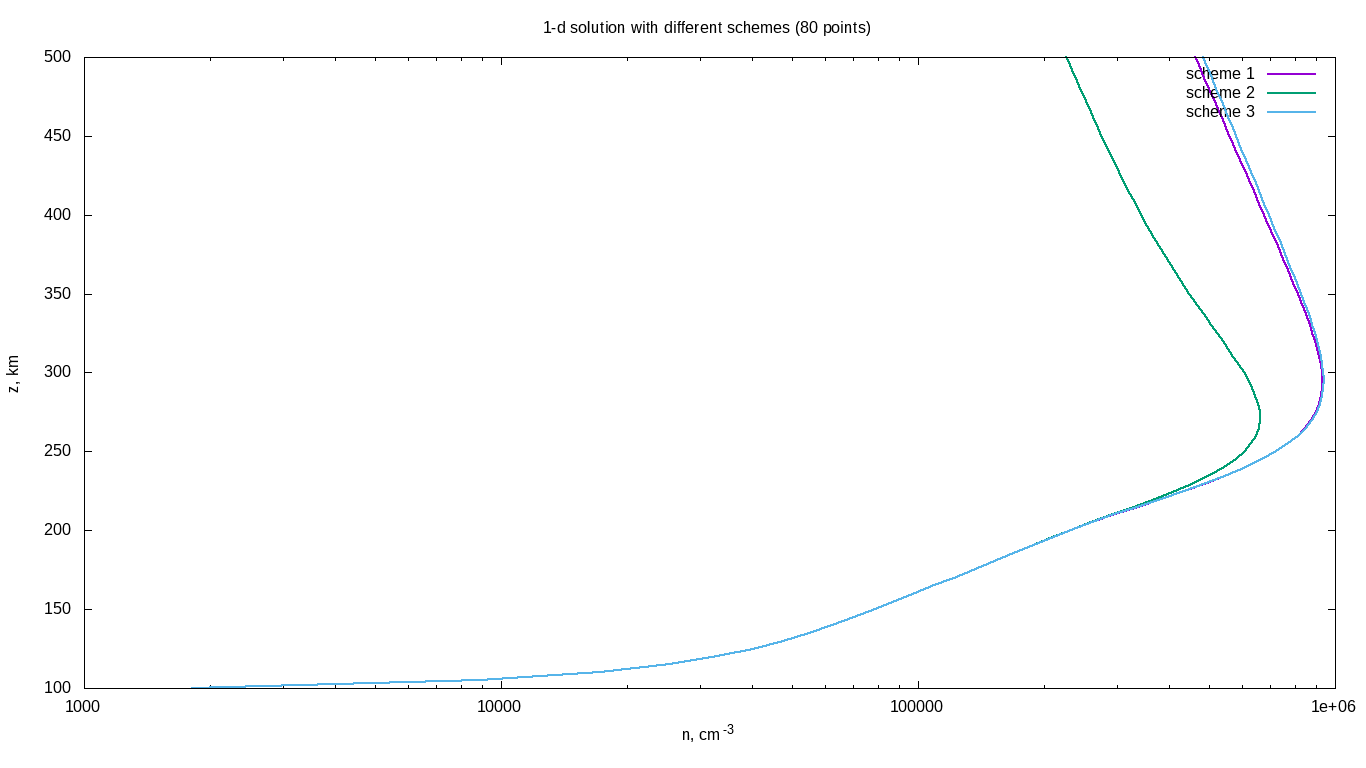
\includegraphics[scale=0.45]{1d_stationary_logscale_80}}
\caption{Стационарные решения на $80$ расчётных узлах.}
\end{figure}

\begin{figure}[H]
\center{
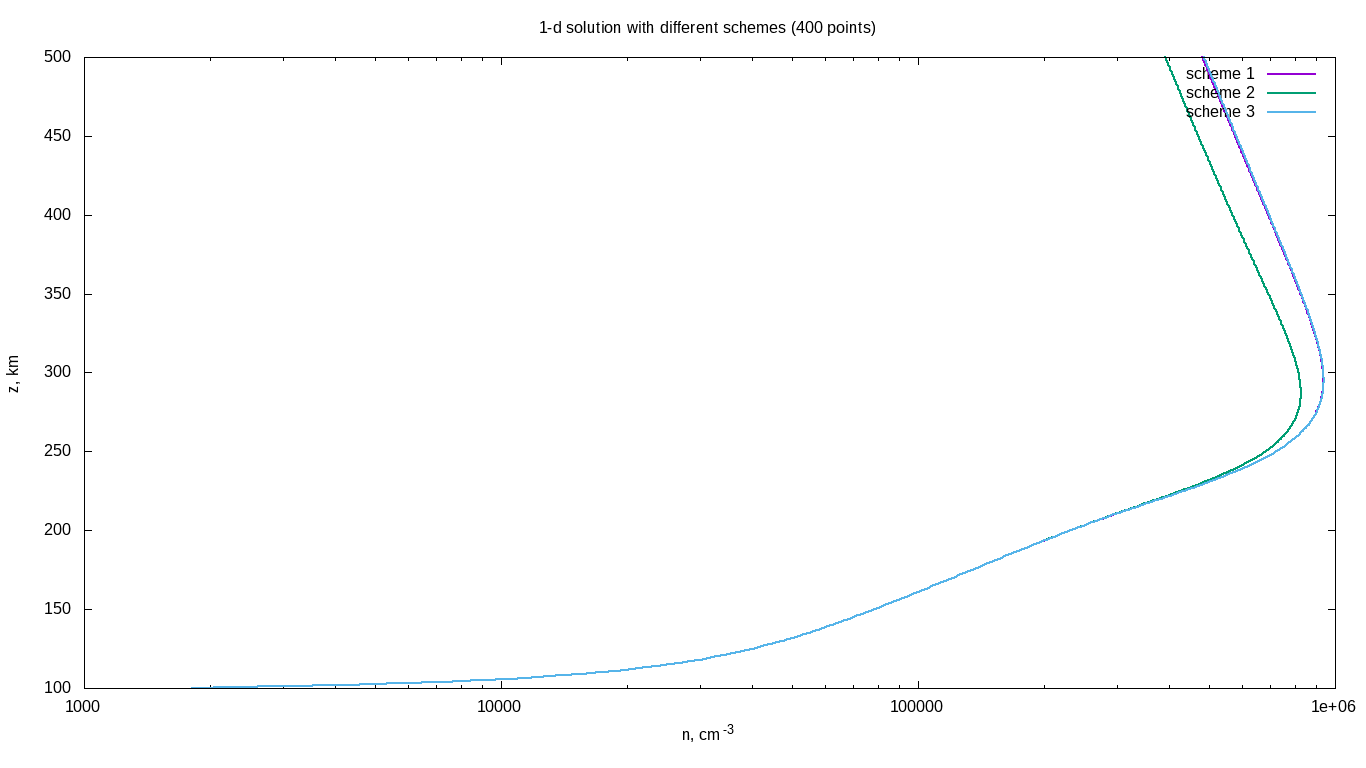
\includegraphics[scale=0.45]{1d_stationary_logscale_400}}
\caption{Стационарные решения на $400$ расчётных узлах.}
\end{figure}

\begin{figure}[H]
\center{
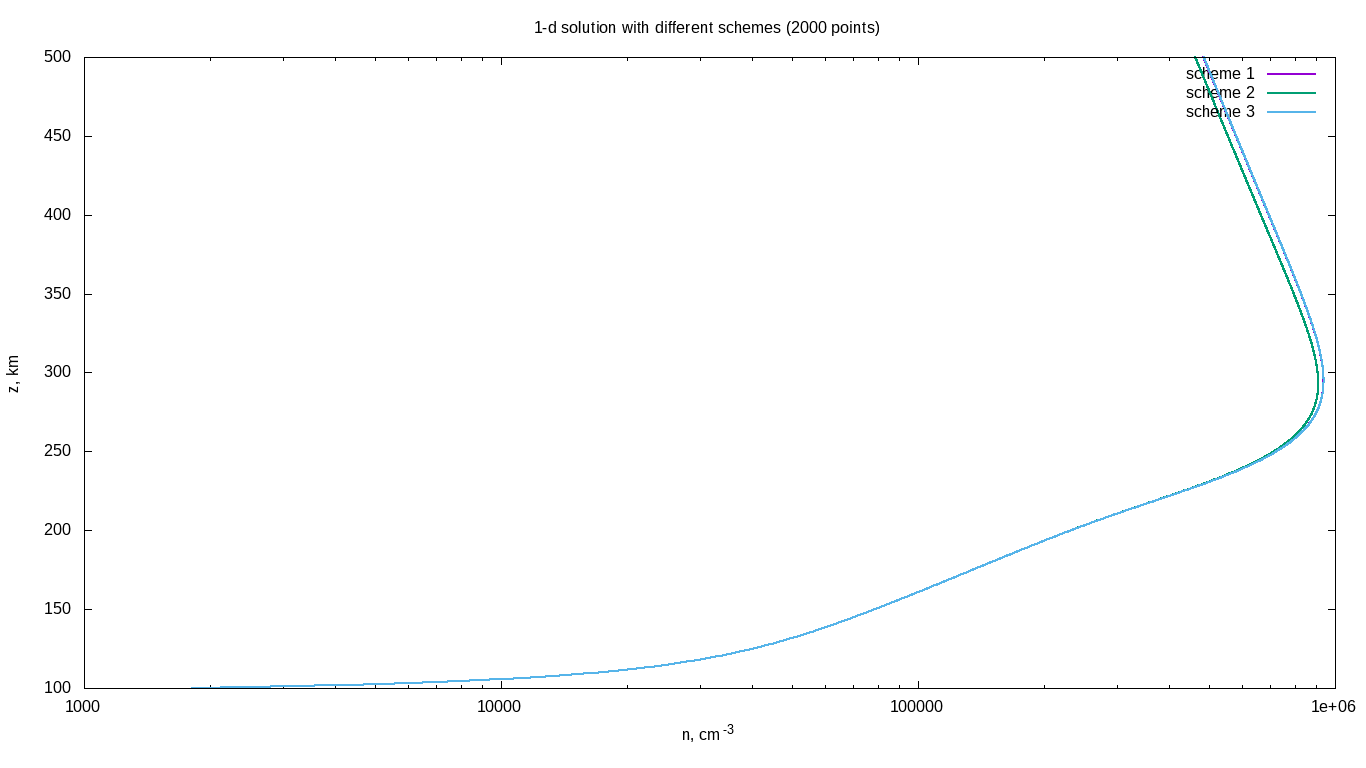
\includegraphics[scale=0.45]{1d_stationary_logscale_2000}}
\caption{Стационарные решения на $2000$ расчётных узлах.}
\end{figure}

\subsection{Чувствительности ко внешним параметрам уравнения}
\subsectionmark{Чувствительности ко внешним параметрам уравнения}



Полученное решение позволяет исследовать чувствительность к изменению различных входящих в уравнение внешних параметров: температурам, концентрациям нейтральных молекул, фотоионизации и рекомбинации. На следующих ниже графиках представлены результаты варьирования каждого из параметров в отдельности на $10\%$ и $20\%$ (в обе стороны). В каждом случае вычислено стационарное решение при изменённом параметре, на всех графиках средняя кривая отвечает невозмущенному уравнению.

\medskip

Варьирование входящих в уравнение температур показывает, что наибольшую чувствительность решение имеет к температуре нейтральных молекул. Изменение концентрации нейтральных молекул~---~атомарного кислорода, молекулярного кислорода и азота показывает, что наибольшая чувствительность решения отвечает изменению концентрации атомарного кислорода, а чувствительности к изменению концентраций атомарного кислорода и азота приблизительно одинаковы.

\medskip

\begin{figure}
\center{
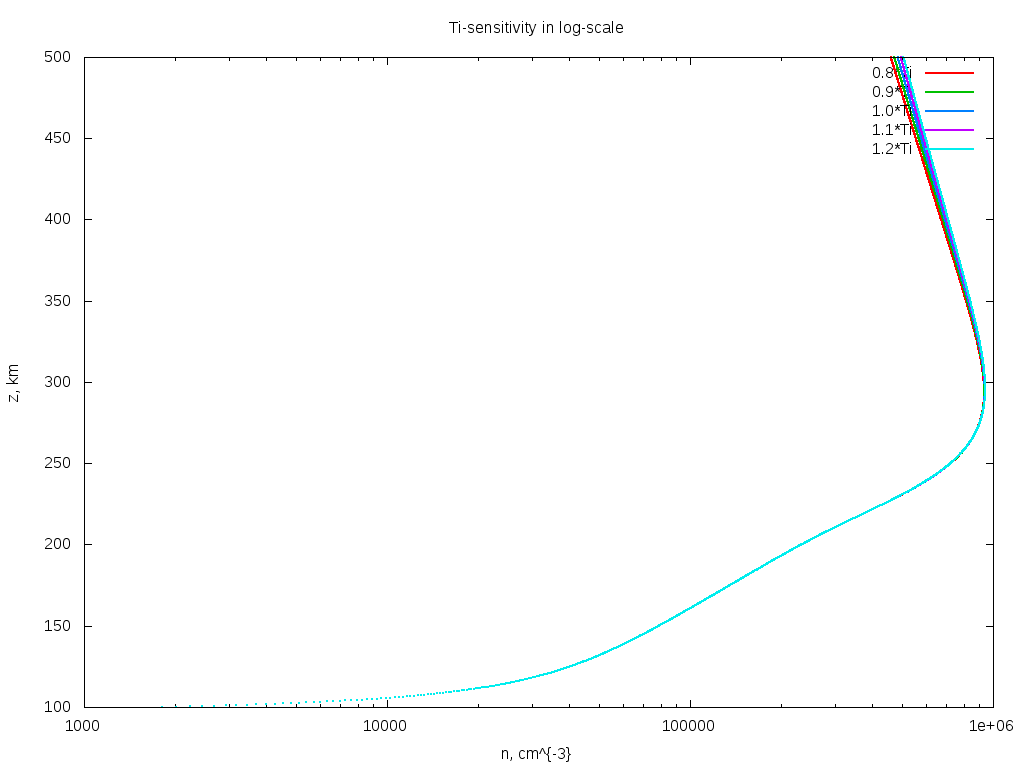
\includegraphics[scale=0.5]{Ti-sensitivity_log}}
\caption{Чувствительность к изменению температуры ионов.}
\end{figure}

\begin{figure}
\center{
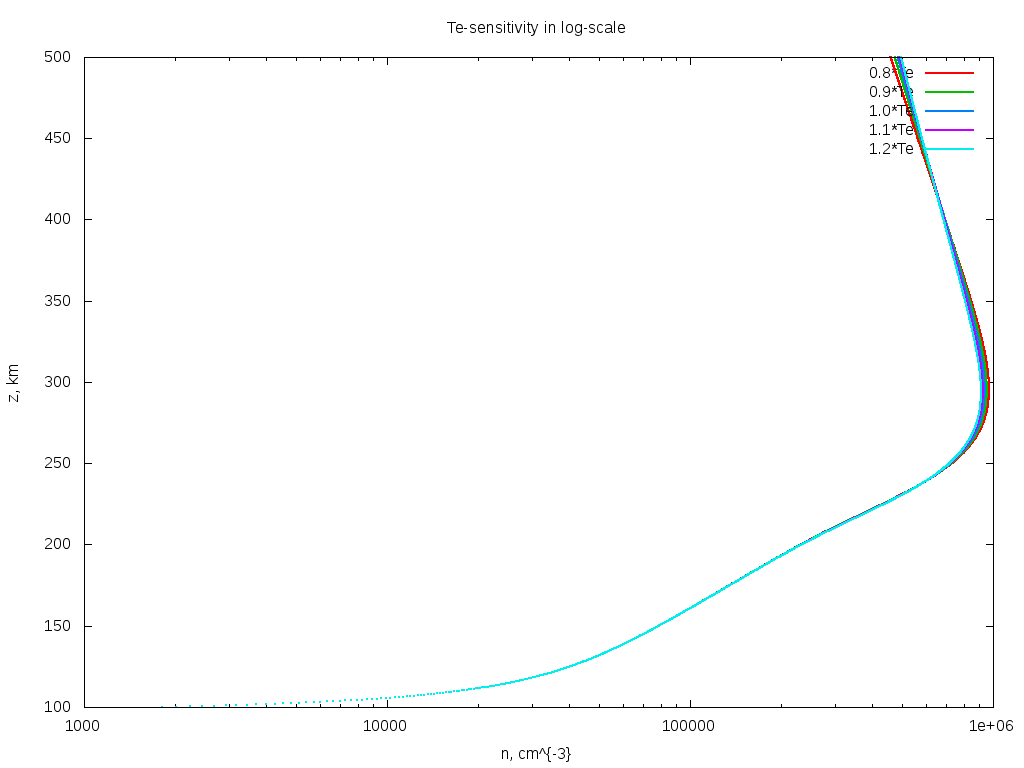
\includegraphics[scale=0.5]{Te-sensitivity_log}}
\caption{Чувствительность к изменению температуры электронов.}
\end{figure}

\begin{figure}
\center{
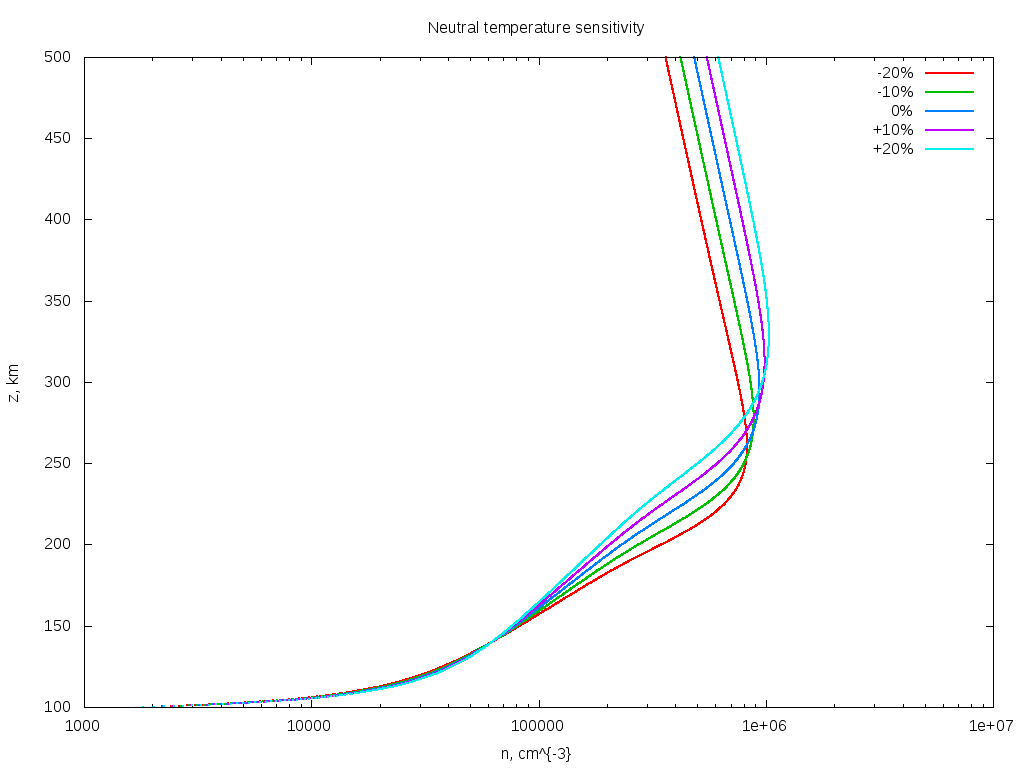
\includegraphics[scale=0.5]{Tn-sensitivity_log}}
\caption{Чувствительность к изменению температуры нейтральных молекул.}
\end{figure}

\begin{figure}
\center{
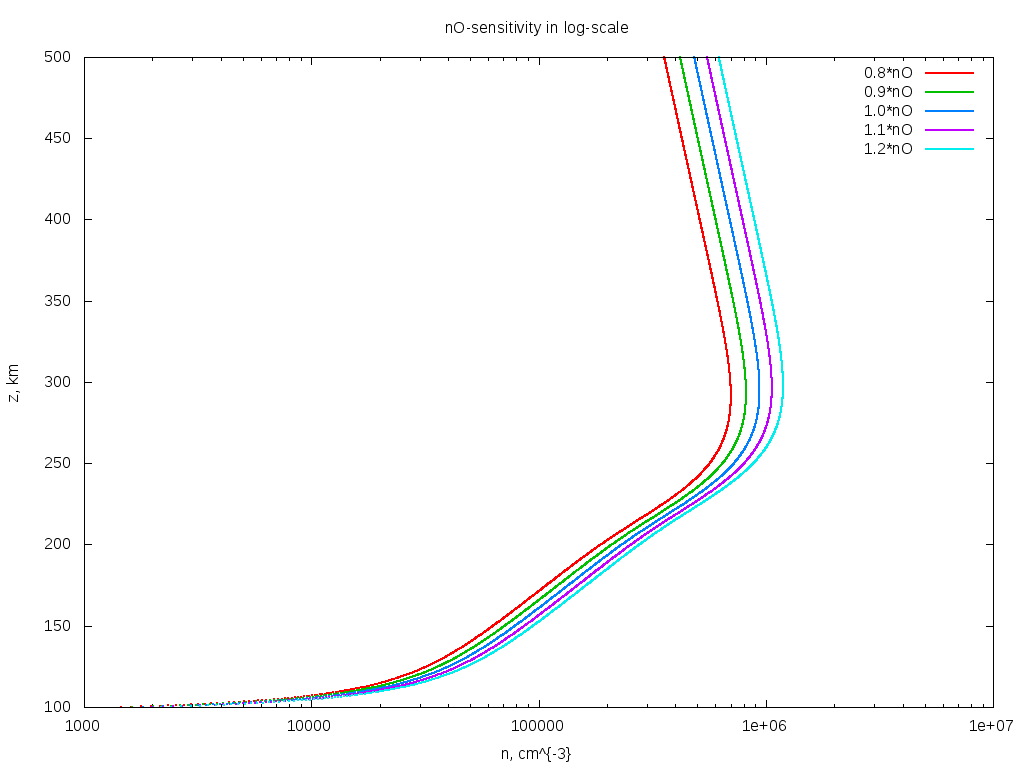
\includegraphics[scale=0.5]{nO-sensitivity_log}}
\caption{Чувствительность к изменению концентрации атомарного кислорода.}
\end{figure}

\begin{figure}
\center{
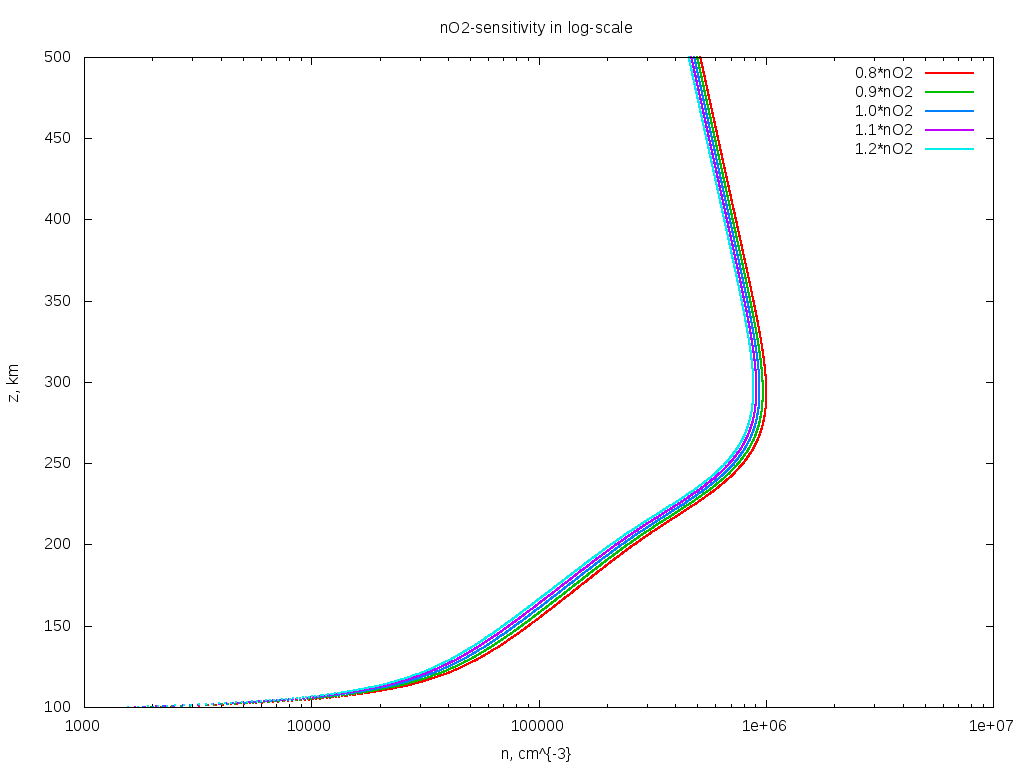
\includegraphics[scale=0.5]{nO2-sensitivity_log}}
\caption{Чувствительность к изменению концентрации молекулярного кислорода.}
\end{figure}

\begin{figure}
\center{
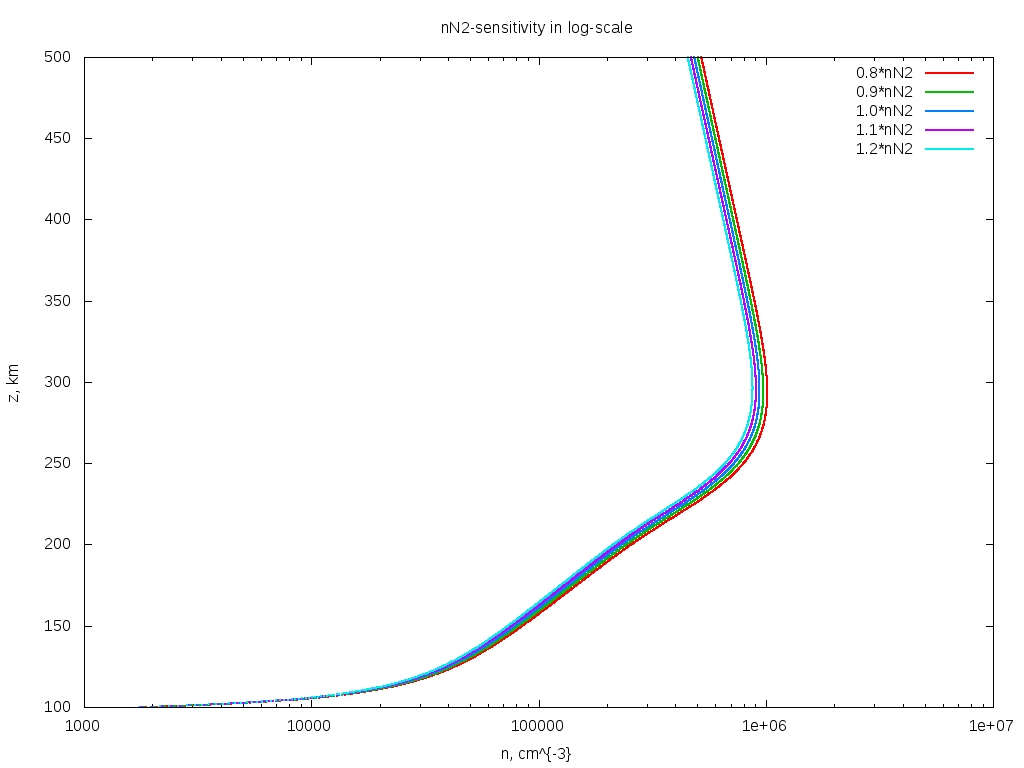
\includegraphics[scale=0.5]{nN2-sensitivity_log}}
\caption{Чувствительность к изменению концентрации азота.}
\end{figure}



%\subsection{Согласованность аппроксимаций граничного условия и уравнения}
%\subsectionmark{Согласованность аппроксимаций граничного условия и уравнения}

%При численном решении квазидвумерного уравнения в предыдущих экспериментах были использованы центральные разности для аппроксимации как уравнения, так и граничного условия. Выясним, каково влияние согласованности этих аппроксимаций на решение: для верхнего граничного условия продолжим использовать центральную разность, а уравнение аппроксимируем, используя для дополнительного слагаемого со смешанной производной аппроксимацию направленными разностями (с учетом знакопеременности скорости): $$\dfrac{|u_\varphi|+u_\varphi}{2}\cdot\dfrac{n_{i+1}-n_i}{h_i} + \dfrac{|u_\varphi|-u_\varphi}{2}\cdot\dfrac{n_{i-1}-n_i}{h_{i-1}}.$$

%Результат численного эксперимента показывает, что при широтах, далёких от нулевой, влияние несущественно, но вблизи экватора решение меняется заметно: 

%\begin{figure}[H]
%\center{
%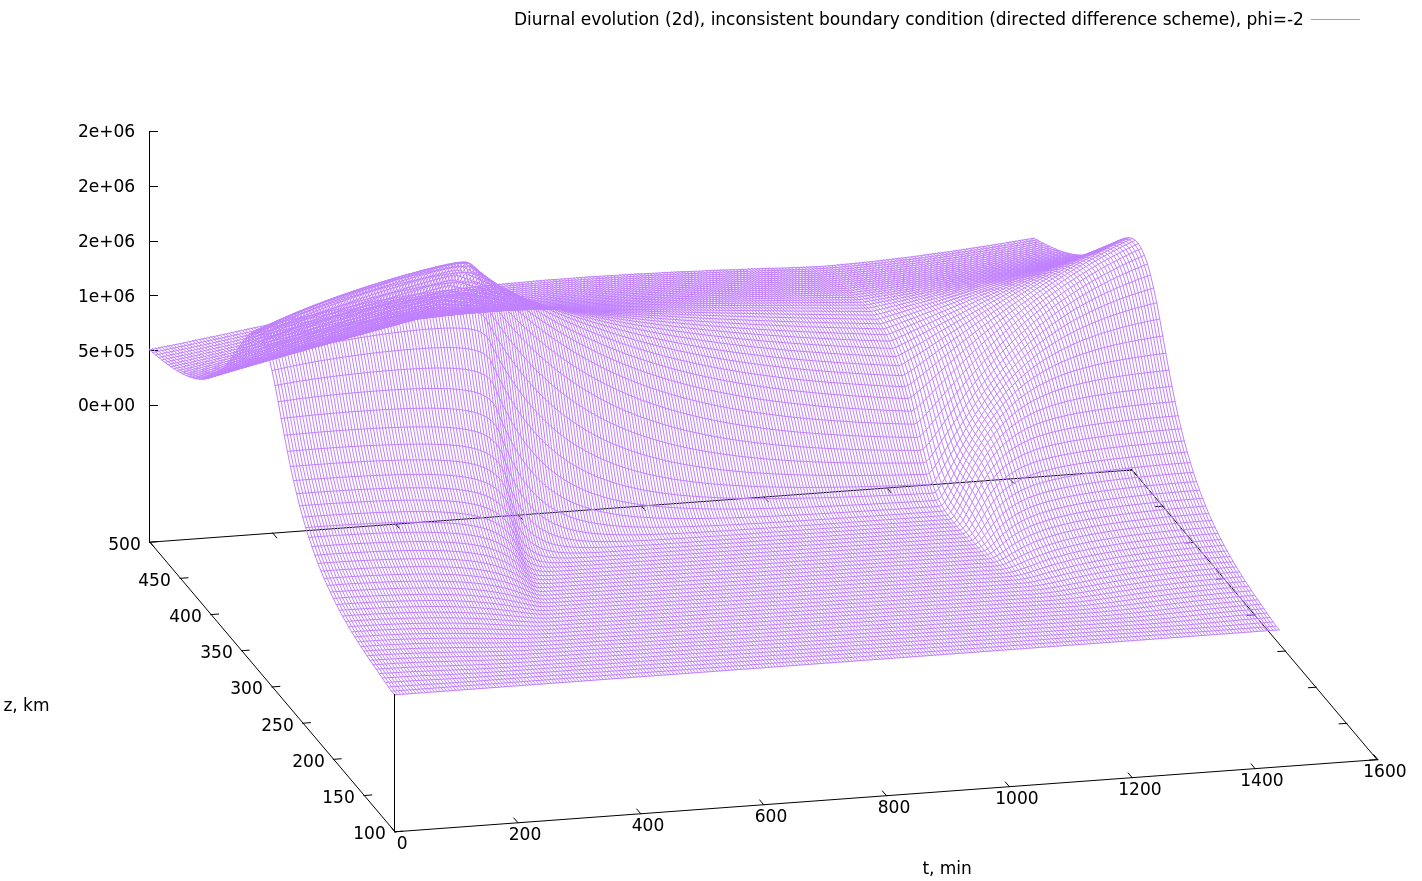
\includegraphics[scale=0.3]{diurnal_2d_inconsistent_boundary_-2}}
%\caption{Использование несогласованных схем для гр. условия и для уравнения, $\varphi = -2^\circ$.}
%\end{figure}


\subsection{Сравнение стационарных решений в различных постановках}
\subsectionmark{Сравнение стационарных решений в различных постановках}


Различные постановки используются для учёта наклонения магнитных силовых линий. Для исследования и сравнения качественных отличий полученных результатов установим не зависящую от времени ионизацию $P(z, t) \equiv P_0(z)$ и изучим сходимости к стационарным решениям с одних и тех же начальных условий~---~вектора с компонентами, равными единице (такой вектор отвечает <<почти нулевому>> решению, при этом даёт возможность использовать схемы, применение которых к случаю нулевых значений затруднено, как, например, в случае логарифма для $u_\varphi$). 

Полученные решения при широтах $\varphi = -88^\circ$, $-66^\circ$, $-50^\circ$, $-40^\circ$, $-30^\circ$, $-16^\circ$, $-2^\circ$, а также и решения при $\varphi = 0^\circ$, соответствующие положению на экваторе, представлены на следующих графиках:

\begin{figure}[H]
\center{
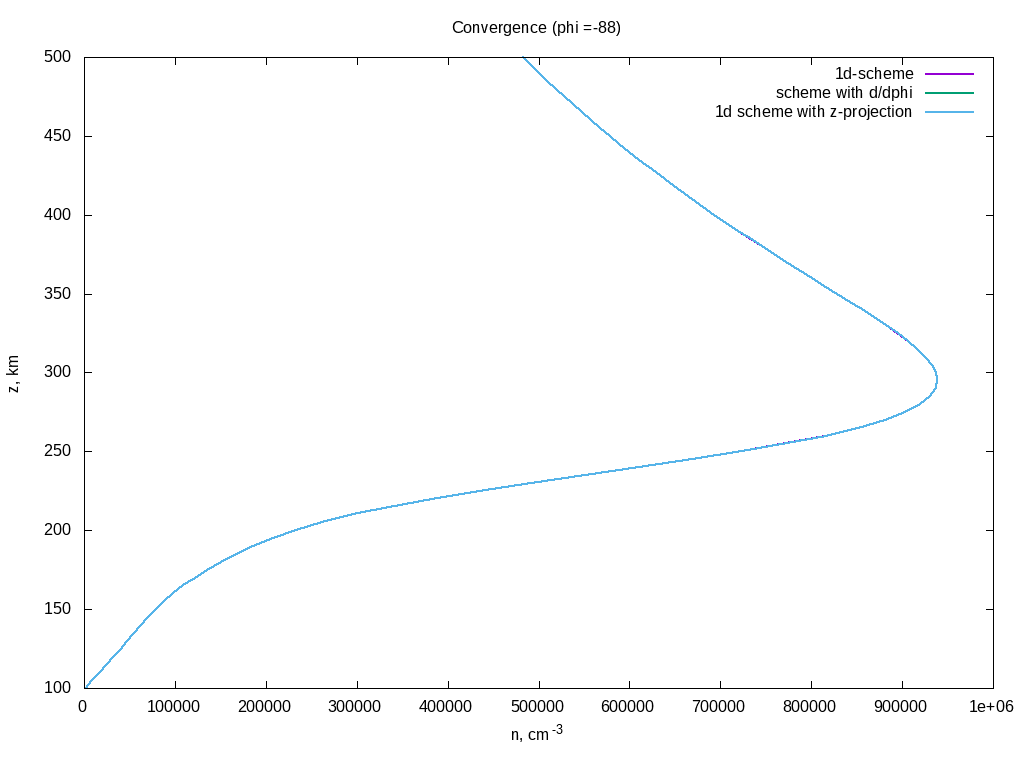
\includegraphics[scale=0.55]{stationary_-88}}
\caption{Стационарные решения для трёх различных постановок, $\varphi = -88^\circ$.}
\end{figure}

\begin{figure}[H]
\center{
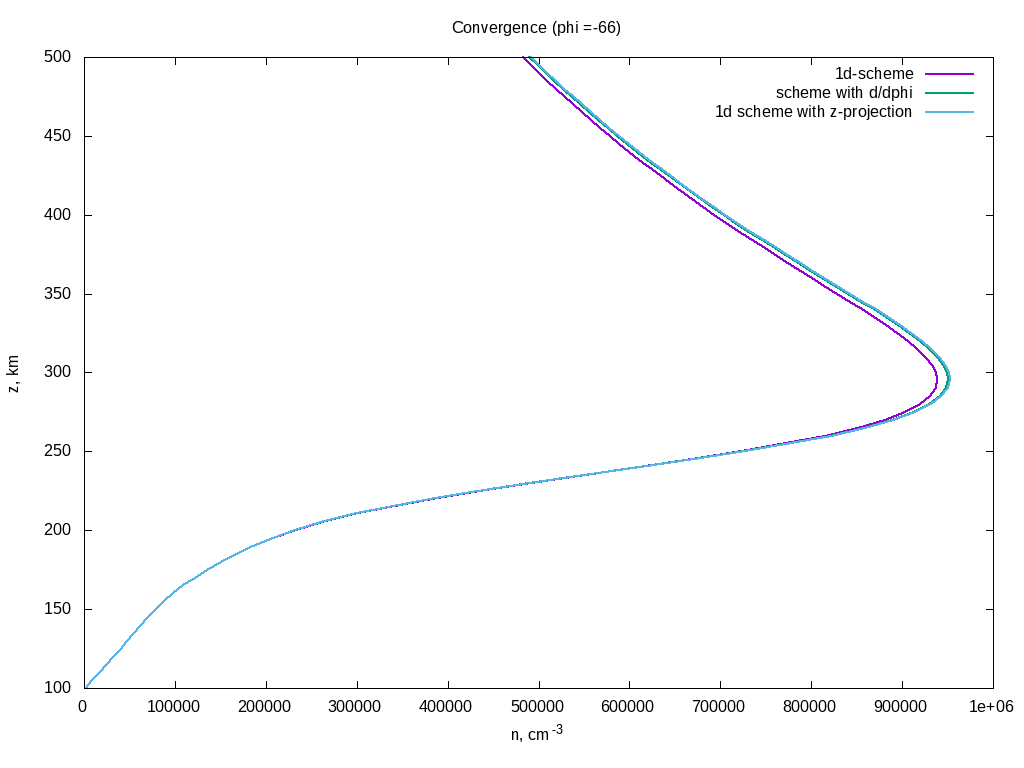
\includegraphics[scale=0.55]{stationary_-66}}
\caption{Стационарные решения для трёх различных постановок, $\varphi = -66^\circ$.}
\end{figure}

\begin{figure}[H]
\center{
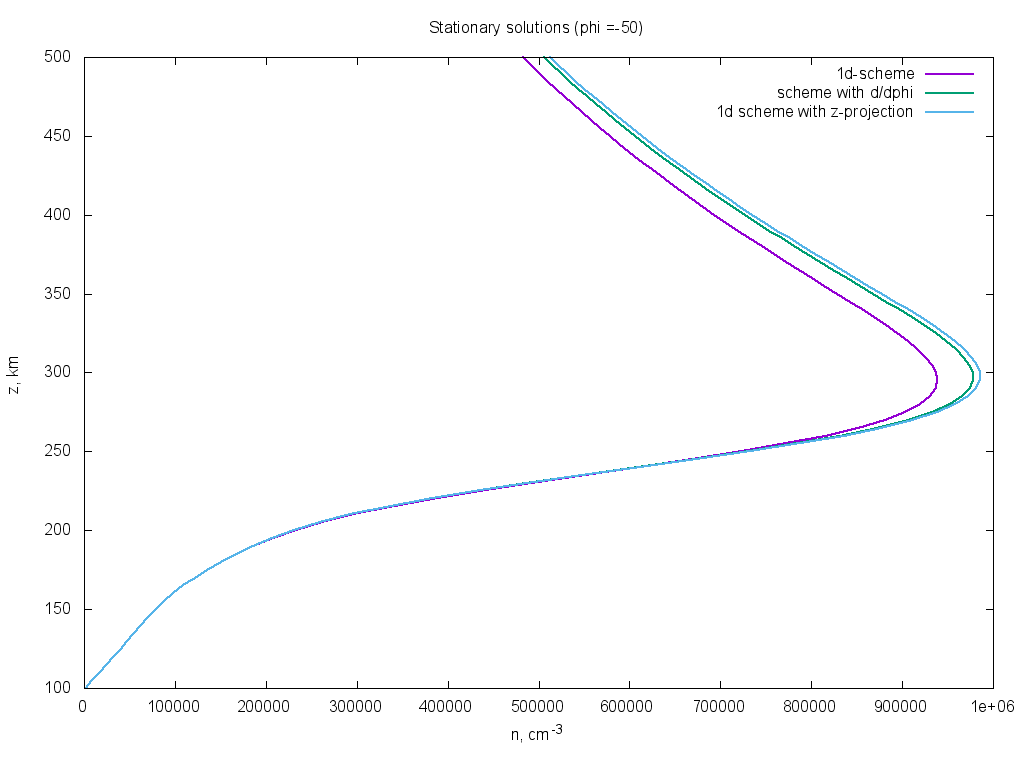
\includegraphics[scale=0.55]{stationary_-50}}
\caption{Стационарные решения для трёх различных постановок, $\varphi = -50^\circ$.}
\end{figure}

\begin{figure}[H]
\center{
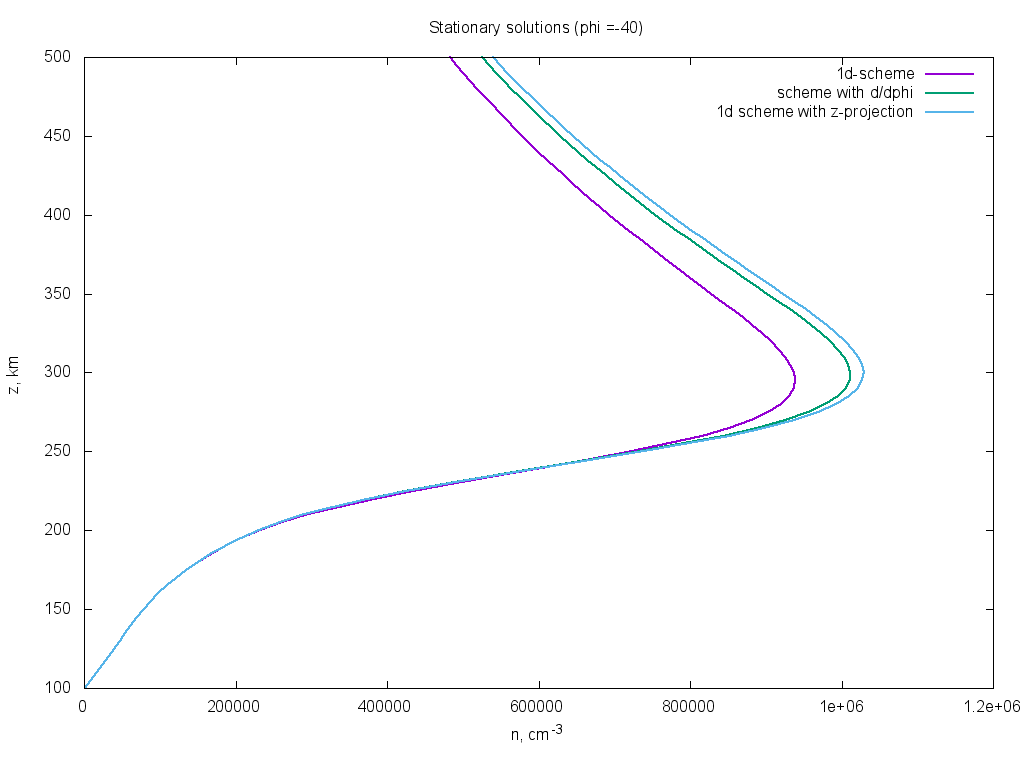
\includegraphics[scale=0.55]{stationary_-40}}
\caption{Стационарные решения для трёх различных постановок, $\varphi = -40^\circ$.}
\end{figure}

\begin{figure}[H]
\center{
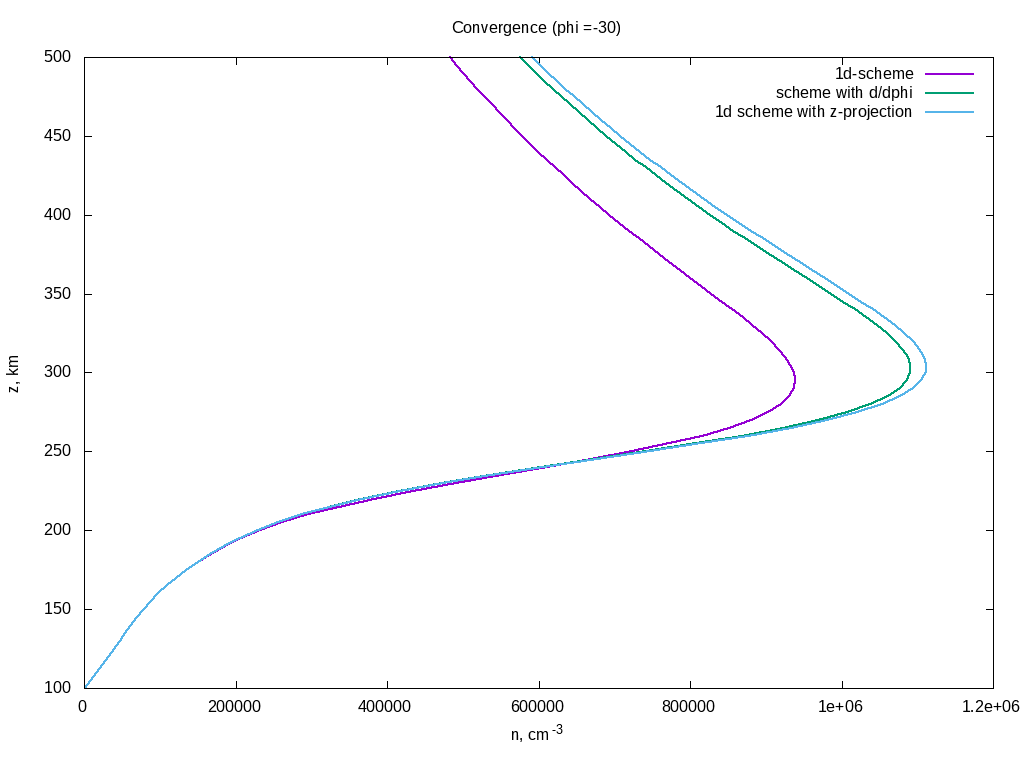
\includegraphics[scale=0.55]{stationary_-30}}
\caption{Стационарные решения для трёх различных постановок, $\varphi = -30^\circ$.}
\end{figure}


\begin{figure}[H]
\center{
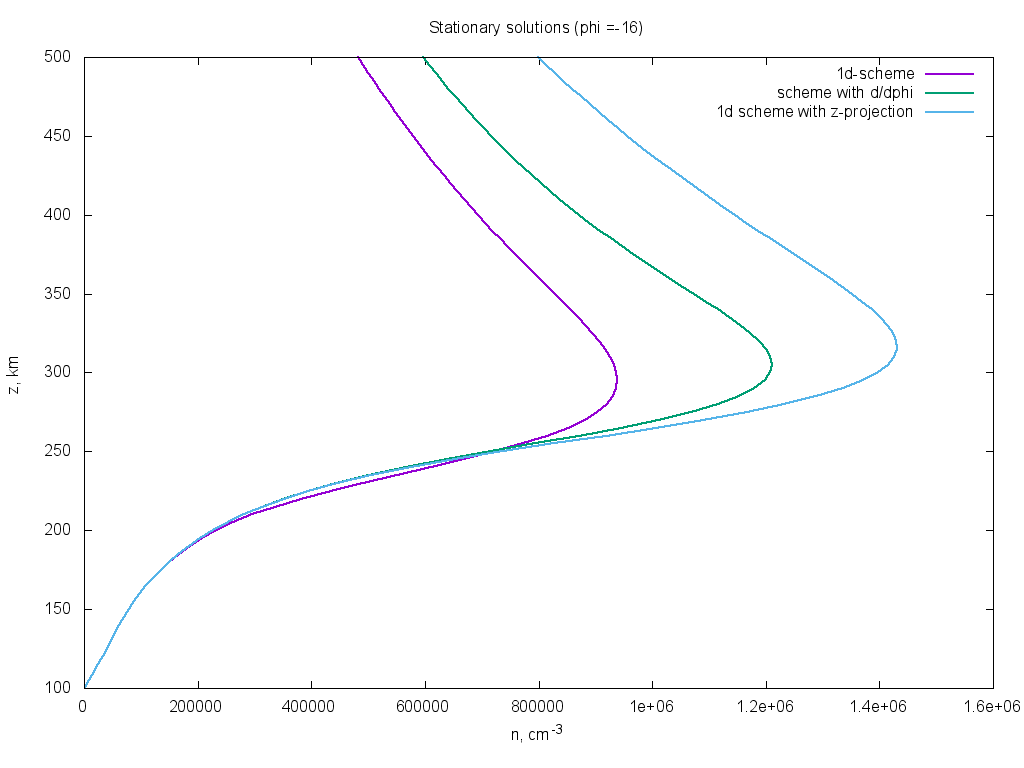
\includegraphics[scale=0.55]{stationary_-16}}
\caption{Стационарные решения для трёх различных постановок, $\varphi = -16^\circ$.}
\end{figure}


\begin{figure}[H]
\center{
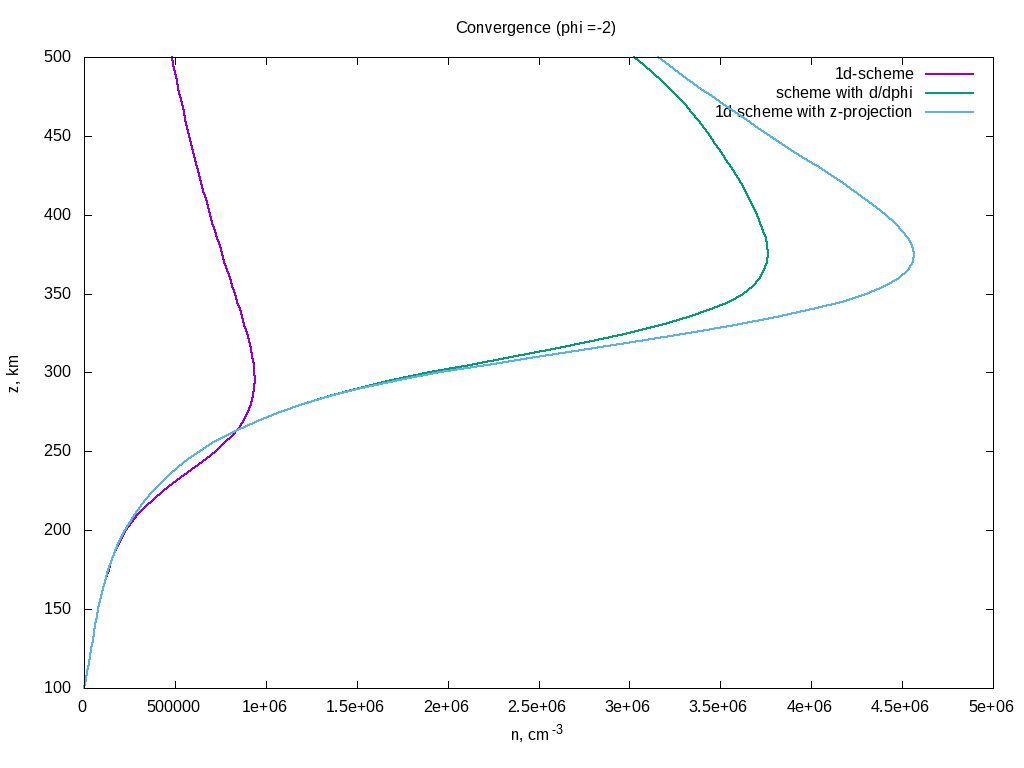
\includegraphics[scale=0.55]{stationary_-2}}
\caption{Стационарные решения для трёх различных постановок, $\varphi = -2^\circ$.}
\end{figure}

\begin{figure}[H]
\center{
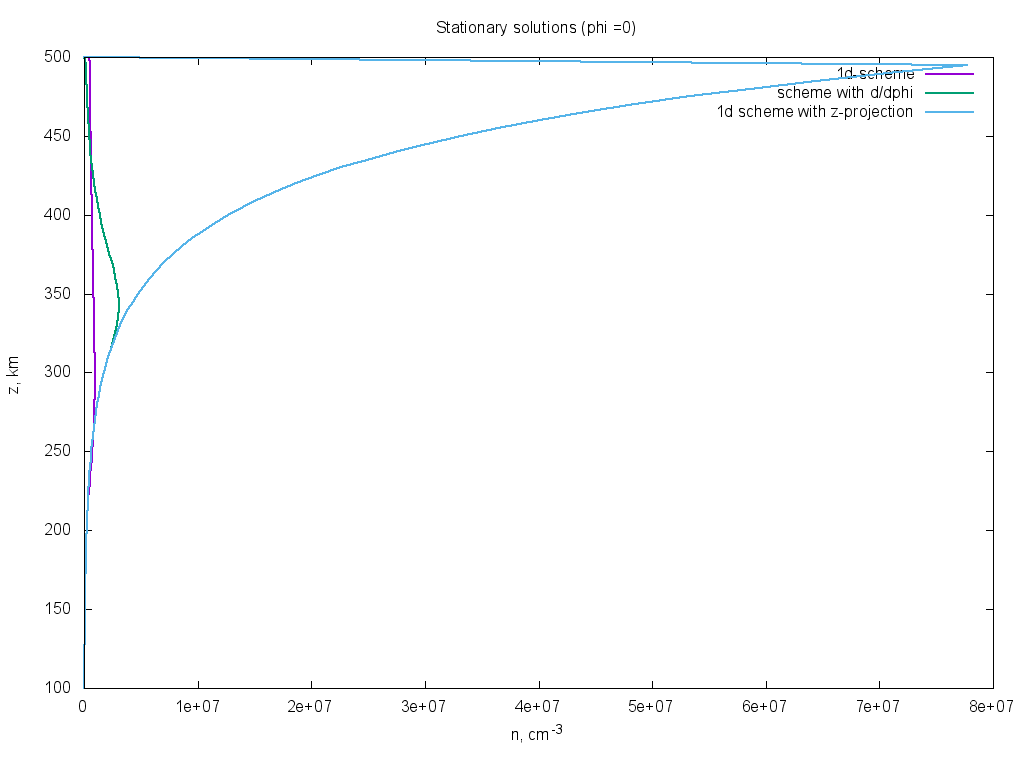
\includegraphics[scale=0.55]{stationary_-0}}
\caption{Стационарные решения для трёх различных постановок, $\varphi = 0^\circ$.}
\end{figure}

Из представленных графиков видно, что решения тем больше отилчаются, чем ближе рассматриваемая широта к экватору. Вблизи полюса все три стационарных решения практически совпадают со стационарным решением одномерной задачи без учёта широтной зависимости. Напротив, вблизи экватора различия весьма существенны: учёт широтной зависимости значительно увеличивает решение по сравнению со стационарным распределением электронной плотности на полюсе. Отметим также, что фактическое получаемое решение на экваторе (при $\varphi = 0^\circ$) в одномерной задаче с проекцией на ось $z$ не соответствует никакому физическому явлению и не описывает действительное распределение электронной плотности. Как уже было упомянуто, при нулевой широте в уравнении обнуляется вся диффузионная часть, а остаются лишь функции фотоионизации и рекомбинации $P$ и $k$, откуда в стационарном случае находим $n_e = \dfrac{P}{k}$, что соответствует экспоненциальному росту концентрации, как если бы единственными процессами в системе были фотохимические процессы.




\subsection{Моделирование суточного хода в одномерной модели}
\subsectionmark{Моделирование суточного хода в одномерной модели}


В ходе численного эксперимента по моделированию суточного хода в одномерной модели вычисляется стационарное решение одномерной задачи при дневном значении $P(z)$, а затем итерации по времени продолжаются с уже меняющимся $P(z, t)$ в соответствии со введённой формулой.

Результаты представлены следующим графиком~---~трёхмерной поверхностью, построенной над плоскостью $(z, t)$.

Видно, что за сутки решение восстанавливается до исходного дневного стационарного решения. Кроме того, после обнуления $P$ при зенитных углах больше $90^\circ$ начинается спад электронной концентрации, сопровождающийся изломом по времени (в соответствующий  момент $P$, входящее в уравнение, также терпит излом).

Отметим также, что при обнулении $P$ распределение электронной плотности падает почти до нуля (начиная со стационарного)  приблизительно за $6$ часов.

\begin{figure}[H]
\center{
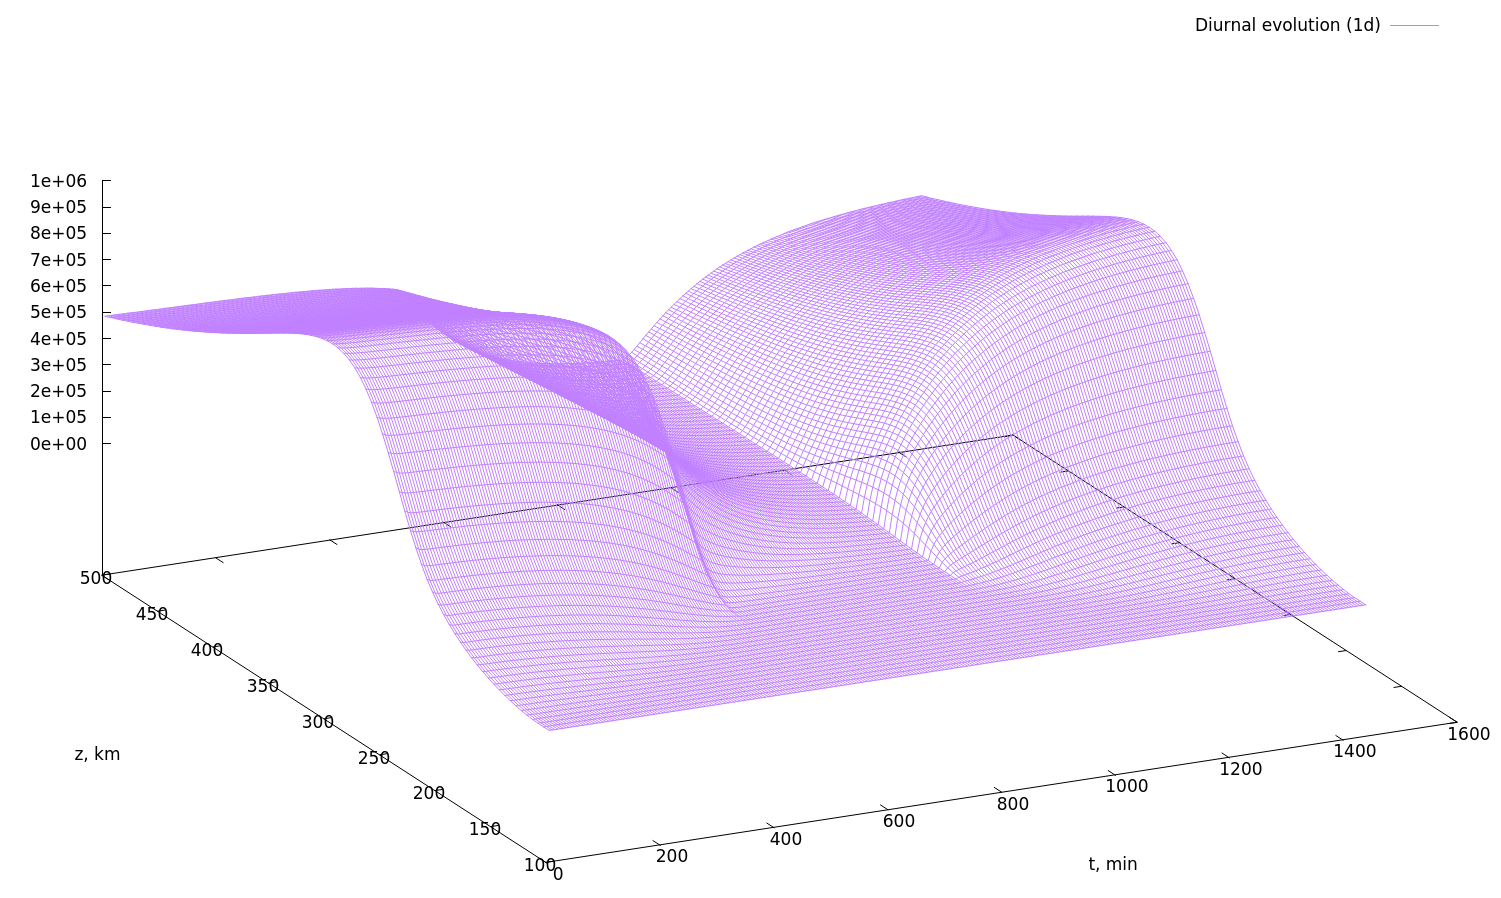
\includegraphics[scale=0.3]{diurnal_1d}}
\caption{Суточный ход в одномерной модели с добавлением зависимости фотоионизации от зенитного угла.}
\end{figure}

\subsection{Суточный ход с учётом широтной зависимости}
\subsectionmark{Суточный ход с учётом широтной зависимости}


Учтём теперь широтную зависимость в уравнении. В качестве первого шага продолжим использование одномерного уравнения, но уже в $z$-проекции, с заменой коэффициента диффузии $D$ на $D\sin^2I$, где $I$~---~угол магнитного наклонения, связанный с широтой $\varphi$ формулой $I\approx \arctg(2\tg \varphi)$.

Как и для одномерного уравнения без широтной зависимости, сначала рассчитываем стационарное решение при дневном значении функции фотоионизации $P$, после чего с итерациями по времени меняем $P$ в соответствии с изменением зенитного угла.

Результаты расчётов суточного хода в одномерной модели с учётом широтной зависимости при широтах $\varphi = -88^\circ, -66^\circ, -30^\circ, -1^\circ$ приведены на следующих графиках:

\begin{figure}[H]
\center{
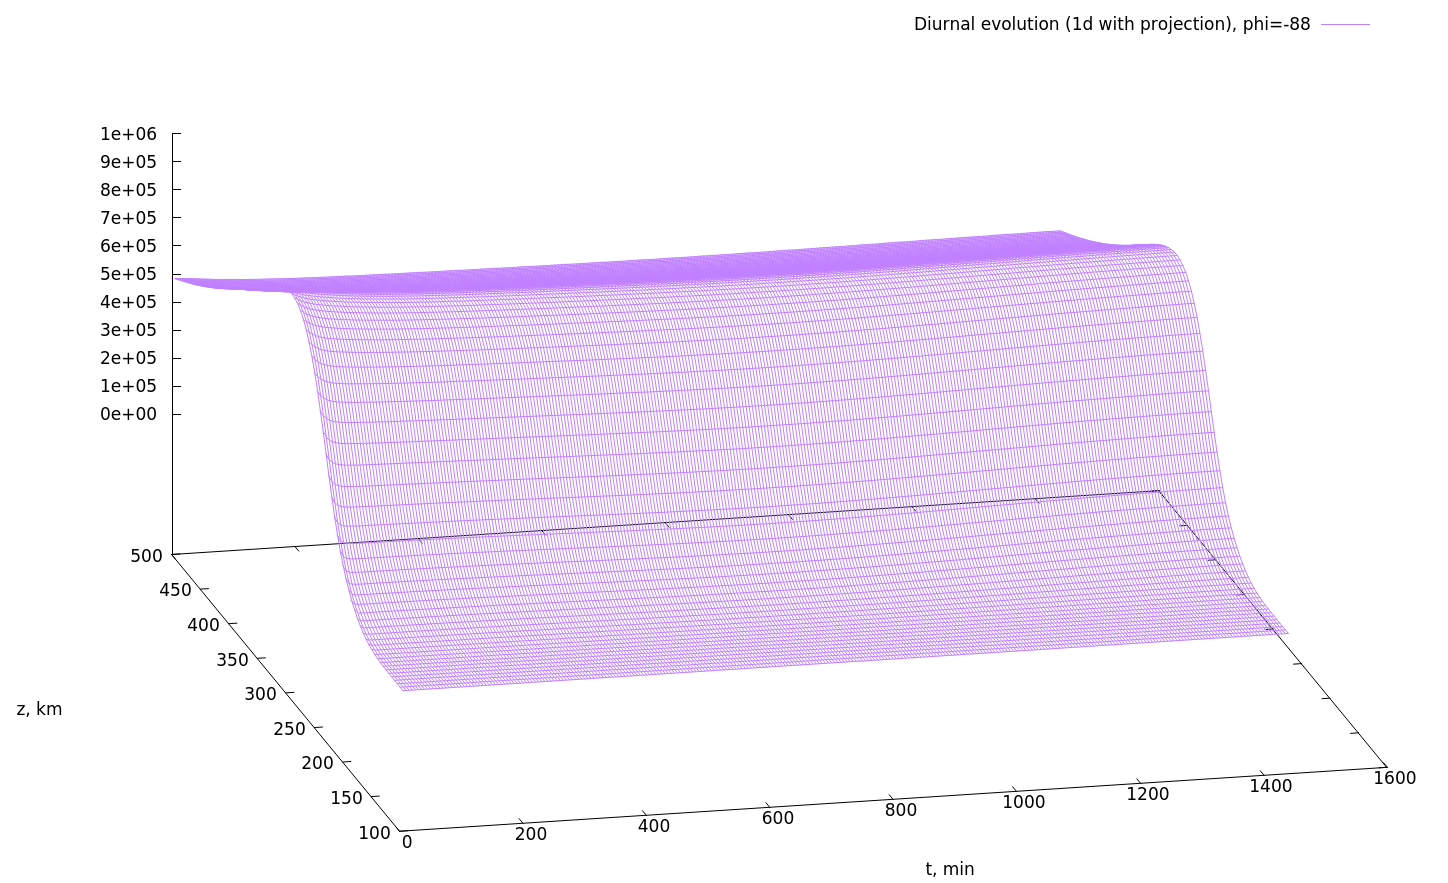
\includegraphics[scale=0.3]{diurnal_projection_-88}}
\caption{Суточный ход в одномерной модели с учётом проекции на магнитную силовую линию, $\varphi = -88^\circ$.}
\end{figure}

\begin{figure}[H]
\center{
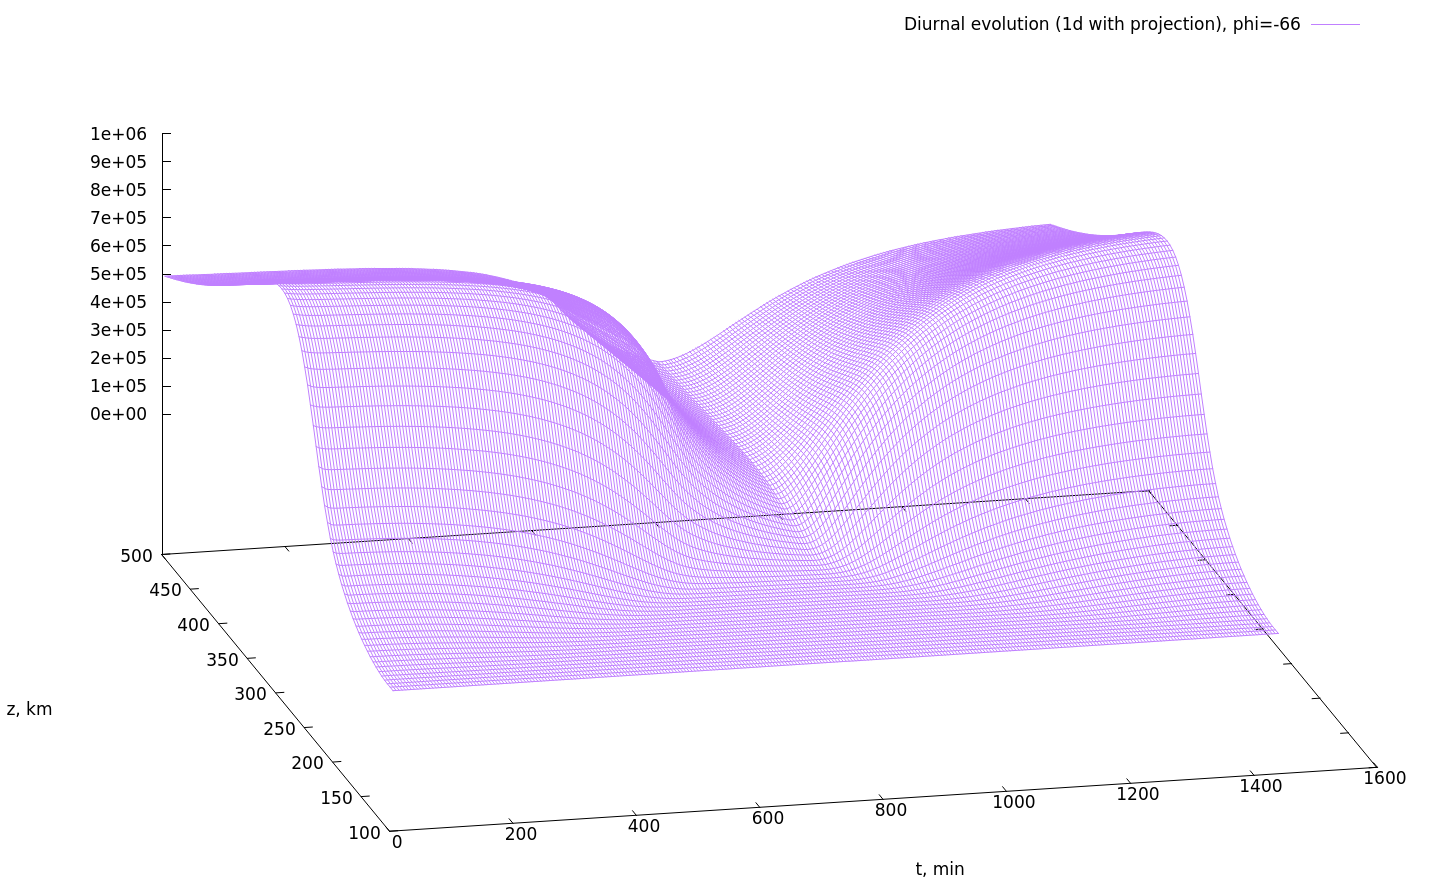
\includegraphics[scale=0.3]{diurnal_projection_-66}}
\caption{Суточный ход в одномерной модели с учётом проекции на магнитную силовую линию, $\varphi = -66^\circ$.}
\end{figure}

\begin{figure}[H]
\center{
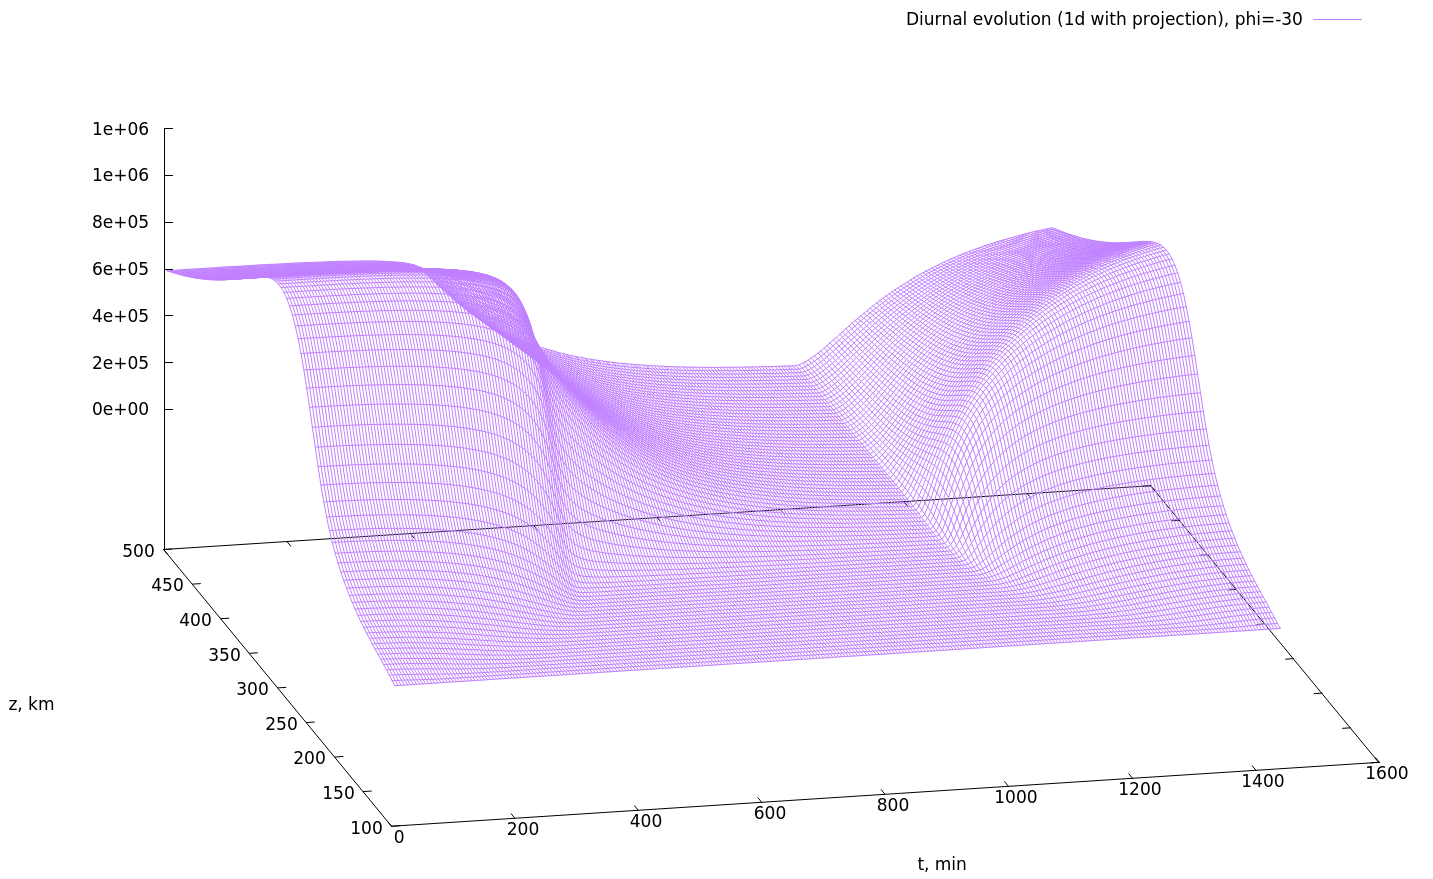
\includegraphics[scale=0.3]{diurnal_projection_-30}}
\caption{Суточный ход в одномерной модели с учётом проекции на магнитную силовую линию, $\varphi = -30^\circ$.}
\end{figure}

\begin{figure}[H]
\center{
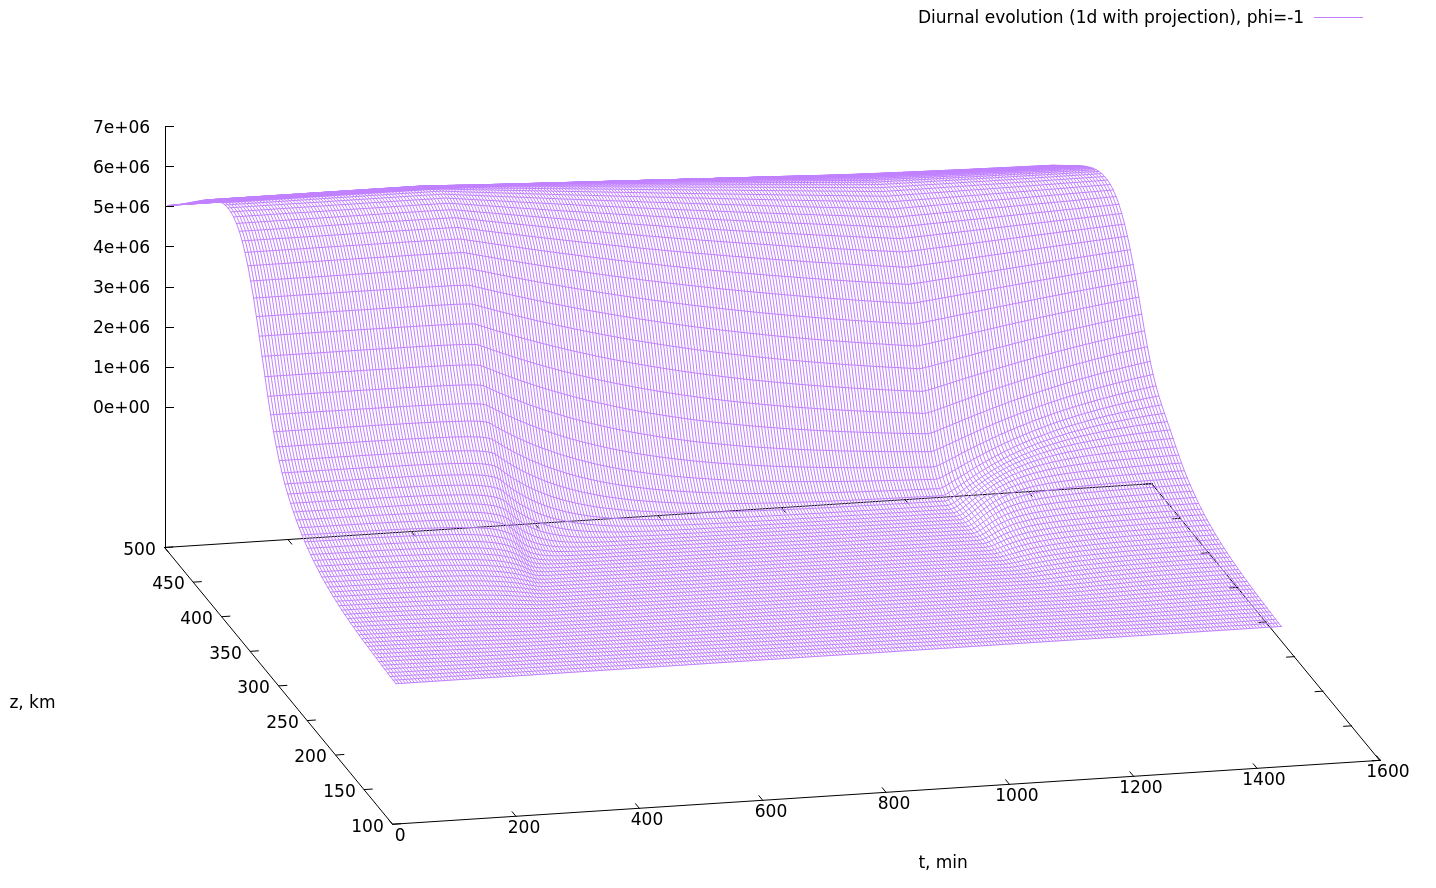
\includegraphics[scale=0.3]{diurnal_projection_-2}}
\caption{Суточный ход в одномерной модели с учётом проекции на магнитную силовую линию, $\varphi = -2^\circ$.}
\end{figure}



Теперь рассмотрим суточный ход в квазидвумерной модели (в $z$-проекции со смешанной производной). На следующих графиках представлен суточный ход при тех же широтах, что и в случае одномерного уравнения с $z$-проекцией. Эксперимент повторяет действия с одномерной моделью: вычисление стационарного дневного решения с последующим изменением функции фотоионизации в согласии с суточным ходом. Существенное отличие наблюдается в характере решения вблизи экватора~---~уравнение не вырождается. 

На графиках приведены результаты моделирования суточного хода в квазидвумерной постановке при широтах $\varphi = 30^\circ$ и $\varphi = -2^\circ$. Качественные отличия от предыдущей постановки становятся заметны именно на широтах вблизи экватора. 


\begin{figure}[H]
\center{
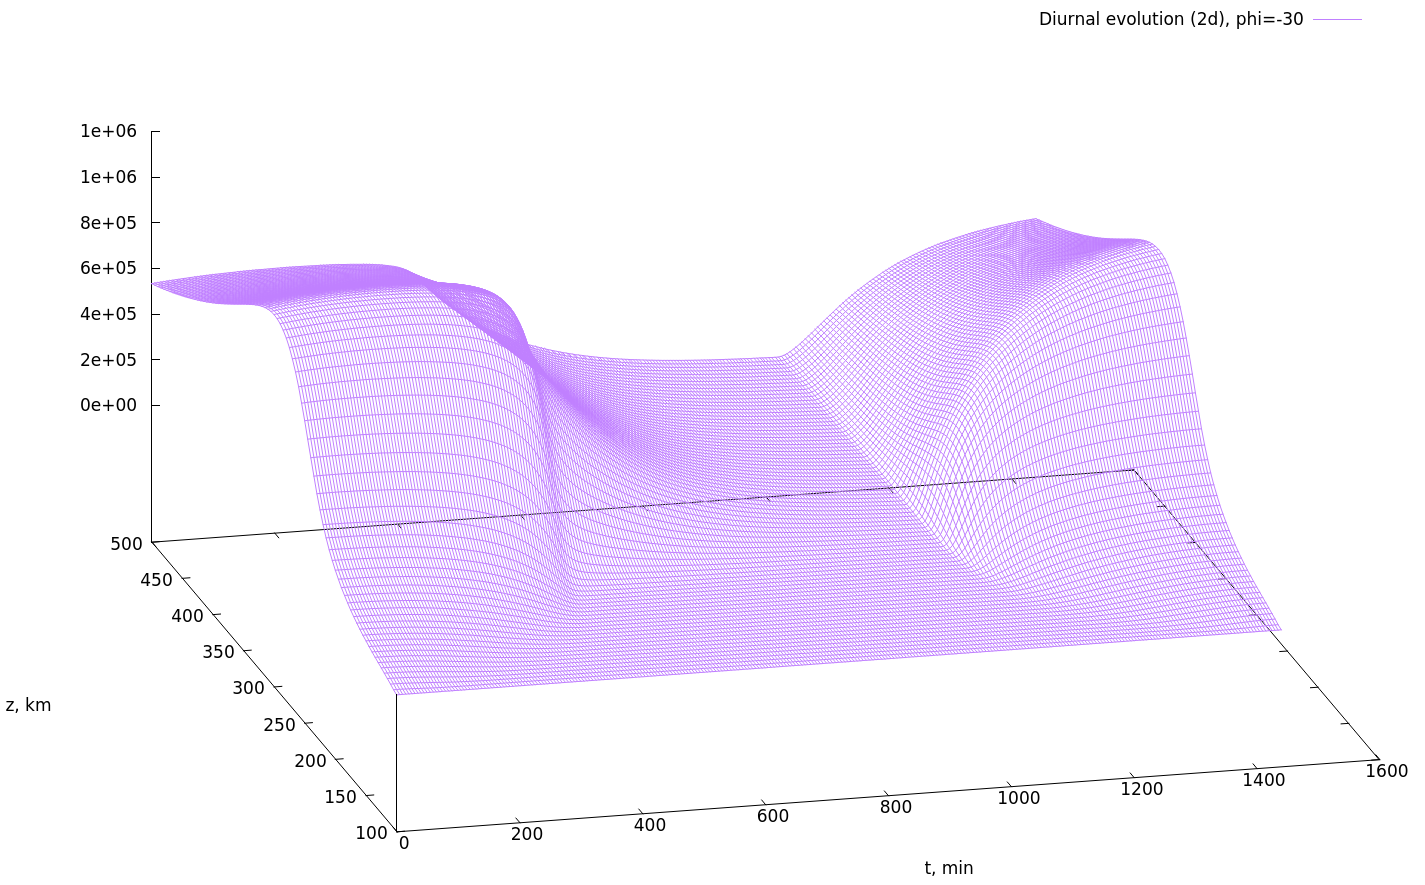
\includegraphics[scale=0.3]{diurnal_2d_-30}}
\caption{Суточный ход в квазидвумерной модели, $\varphi = -30^\circ$.}
\end{figure}

\begin{figure}[H]
\center{
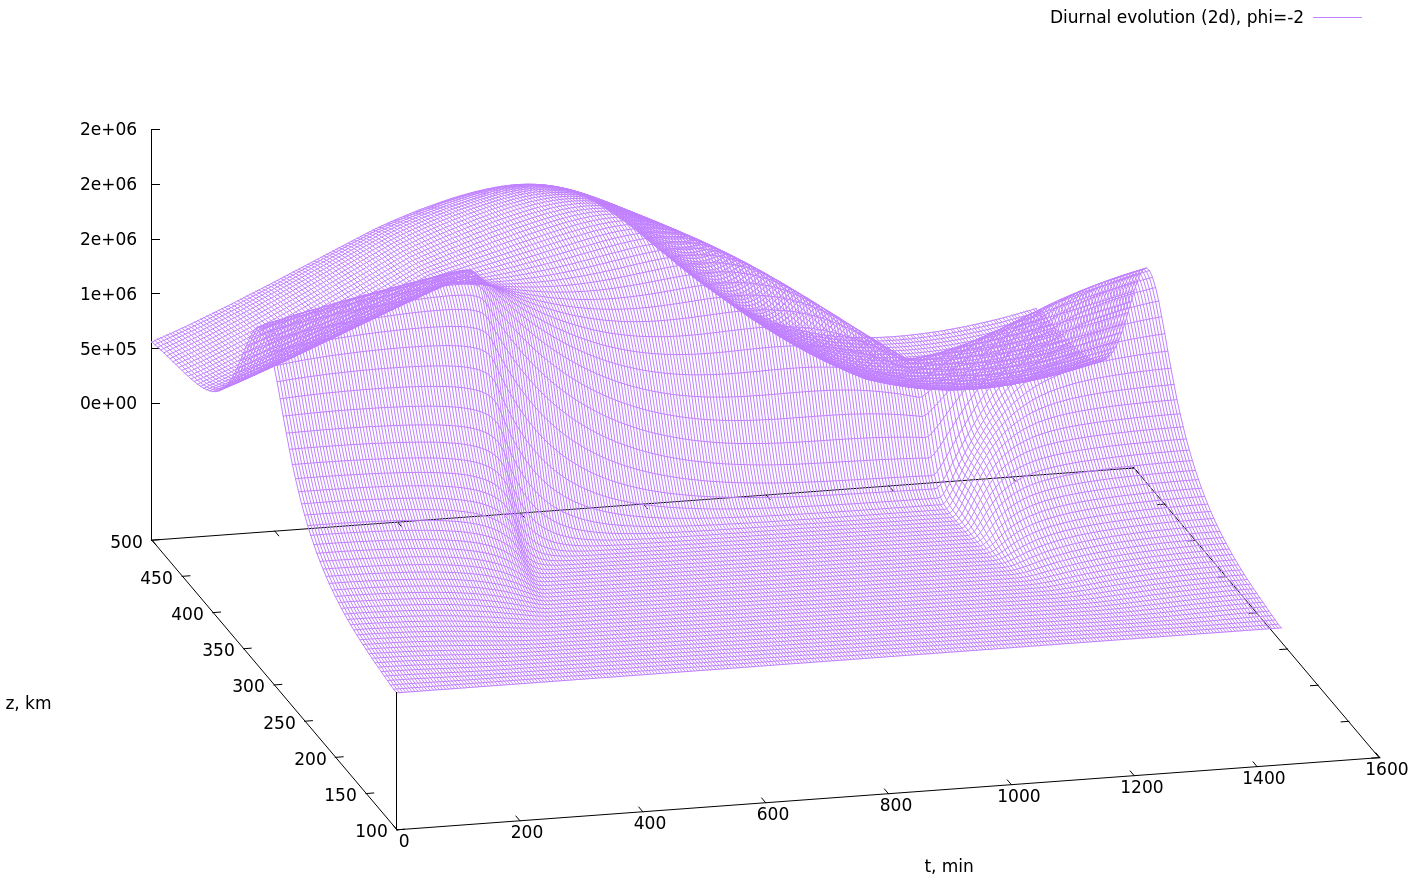
\includegraphics[scale=0.3]{diurnal_2d_-2}}
\caption{Суточный ход в одномерной модели с учётом проекции на магнитную силовую линию, $\varphi = -2^\circ$.}
\end{figure}

\newpage

\section{Заключение}
\sectionmark{Заключение}

Построена трёхмерная динамическая модель ионосферы, в которой с помощью трёхмерного уравнения неразрывности описывается эволюция электронной плотности в $F$-слое.

К векторному уравнению после записи в сферических координатах (в приближении тонкого сферического слоя) применён метод расщепления по физическим процессам и геометрическим переменным. После этого исследовано и численно промоделировано приближенное уравнение, представляющее собой первый шаг метода расщепления. В качестве этапов построения решения поставленной приближённой задачи рассмотрены одномерные и двумерные постановки, учитывающие основные процессы~---~амбиполярную диффузию и процессы фотохимии. Полученные решения применимы при описании ионосферы в средних широтах и вблизи полюсов при отсутствии возмущений.

Для рассмотренных одномерных и двумерной постановок исследованы особенности рассматриваемых дифференциальных уравнений: баланс массы, сильная жесткость решаемых задач, неотрицательность концентрации. Построены разностные схемы, учитывающие эти особенности, получены стационарные профили, промоделирован суточный ход. Для двумерного уравнения применена аппроксимация, позволяющая свести его к одномерному и использовать уже имеющийся программный код: смешанная производная при этом считается эффективной добавкой к скорости переноса.

В результате численных экспериментов проведён сравнительный анализ высотных профилей электронной концентрации, полученных в различных постановках, при различных широтах. Исследована также и чувствительность дневного высотного профиля к изменению величин, входящих в уравнение в качестве внешних параметров.

Анализ полученных численных решений показывает необходимость решения полного трёхмерного уравнения, в частности~---~вблизи экватора, где магнитное поле близко к вертикальному.

План дальнейшего исследования включает в себя решение полной трёхмерной задачи, интеграцию построенной модели в уже разработанную в ИВМ модель термосферы, а также последующее улучшение используемых методов и уточнение результатов.

\newpage
\addcontentsline{toc}{section}{Список использованных источников}

\begin{thebibliography}{00}
\bibitem{KulyaminDyminkov1}
\textit{Kulyamin, D. V. and V. P. Dymnikov.} A three-dimensional model of general thermospheric circulation. // Russian Journal of Numerical Analysis and Mathematical Modelling. 2013. 28(4): 353-380.
\bibitem{KulyaminDymnikov2}
\textit{Кулямин Д.~В., Дымников В.~П.}, Моделирование климата нижней ионосферы. // Известия Российской академии наук. Физика атмосферы и океана, 2015. Т. 51(3): С. 317–337.
\bibitem{Schunk}
\textit{Schunk, R.W. and A.F. Nagy}, IONOSPHERES Physics, Plasma Physics, and Chemistry. 2009, New York, United States: Cambridge University Press.
\end{thebibliography}


\end{document}



